%! Suppress = LineBreak
%! Suppress = TooLargeSection
%%%%%%%%%%%%%%%%%%%%%%%%%%%%%%%%%%%%%%%%%%
%                                        %
% Szablon pracy dyplomowej magisterskiej %
%                                        %
%%%%%%%%%%%%%%%%%%%%%%%%%%%%%%%%%%%%%%%%%%



\documentclass[a4paper,twoside,12pt]{book}
\usepackage[utf8]{inputenc}
\usepackage[T1]{fontenc}
\usepackage{amsmath,amsfonts,amssymb,amsthm}
\usepackage[british,polish]{babel}
\usepackage{indentfirst}
\usepackage{lmodern}
\usepackage{graphicx}
\usepackage{hyperref}
\usepackage{booktabs}
\usepackage{tikz}
\usepackage{pgfplots}
\usepackage{mathtools}
\usepackage[page]{appendix} % toc,
\renewcommand{\appendixtocname}{Dodatki}
\renewcommand{\appendixpagename}{Dodatki}
\renewcommand{\appendixname}{Dodatek}

\usepackage{setspace}
\onehalfspacing


\frenchspacing

\usepackage{listings}
\lstset{
language={},
basicstyle=\ttfamily,
keywordstyle=\lst@ifdisplaystyle\color{blue}\fi,
commentstyle=\color{gray}
}

%%%%%%%%%

%%%% LIST GENERATOR %%%%%%%%%

%\usepackage{tikz}
%\usepackage{manfnt}   % dangerous sign
\usepackage{color}
\definecolor{brickred}      {cmyk}{0 , 0.89, 0.94, 0.28}

\makeatletter \newcommand \kslistofremarks{\section*{Uwagi} \@starttoc{rks}}
\newcommand\l@uwagas[2]
{\par\noindent \textbf{#2:} %\parbox{10cm}
{#1}\par} \makeatother


\newcommand{\ksremark}[1]{%
{%\marginpar{\textdbend}
{\color{brickred}{[#1]}}}%
\addcontentsline{rks}{uwagas}{\protect{#1}}%
}

\newcommand{\comma}{\ksremark{przecinek}}
\newcommand{\nocomma}{\ksremark{bez przecinka}}
\newcommand{\styl}{\ksremark{styl}}
\newcommand{\ortografia}{\ksremark{ortografia}}
\newcommand{\fleksja}{\ksremark{fleksja}}
\newcommand{\pauza}{\ksremark{pauza `--', nie dywiz `-'}}
\newcommand{\kolokwializm}{\ksremark{kolokwializm}}

%%%%%%%%%%%%%% END OF GENERATOR %%%%%%%%%%%

%%%%%%%%%%%% ZYWA PAGINA %%%%%%%%%%%%%%%
% brak kapitalizacji zywej paginy
\usepackage{fancyhdr}
\pagestyle{fancy}
\fancyhf{}
\fancyhead[LO]{\nouppercase{\it\rightmark}}
\fancyhead[RE]{\nouppercase{\it\leftmark}}
\fancyhead[LE,RO]{\it\thepage}


\fancypagestyle{tylkoNumeryStron}{%
\fancyhf{}
\fancyhead[LE,RO]{\it\thepage}
}

\fancypagestyle{NumeryStronNazwyRozdzialow}{%
\fancyhf{}
\fancyhead[LO]{\nouppercase{\it\rightmark}}
\fancyhead[RE]{\nouppercase{\it\leftmark}}
\fancyhead[LE,RO]{\it\thepage}
}


%%%%%%%%%%%%% OBCE WTRETY
\newcommand{\obcy}[1]{\emph{#1}}
\newcommand{\ang}[1]{{\selectlanguage{british}\obcy{#1}}}
%%%%%%%%%%%%%%%%%%%%%%%%%%%%%

% polskie oznaczenia funkcji matematycznych
\renewcommand{\tan}{\operatorname {tg}}
\renewcommand{\log}{\operatorname {lg}}

% jeszcze jakies drobiazgi

\newcounter{stronyPozaNumeracja}

\newcommand{\hcancel}[1]{%
\tikz[baseline=(tocancel.base)]{
\node[inner sep=0pt,outer sep=0pt] (tocancel) {#1};
\draw[red] (tocancel.south west) -- (tocancel.north east);
}%
}%

\newcommand{\miesiac}{%
\ifcase\the\month
\or styczeń% 1
\or luty% 2
\or marzec% 3
\or kwiecień% 4
\or maj% 5
\or czerwiec% 6
\or lipiec% 7
\or sierpień% 8
\or wrzesień% 9
\or październik% 10
\or listopad% 11
\or grudzień% 12
\fi}


%%%%%%%%%%%%%%%%%%%%%%%%%%%%%%%%%%%%%%%%%%%%%%
%%%%%%%%%%%%%%%%%%%%%%%%%%%%%%%%%%%%%%%%%%%%%%
%%%%%%%%%%%%%%%%%%%%%%%%%%%%%%%%%%%%%%%%%%%%%%
%%%%%%%%%%%%%%%%%%%%%%%%%%%%%%%%%%%%%%%%%%%%%%
%%%%%%%%%%%%%%%%%%%%%%%%%%%%%%%%%%%%%%%%%%%%%%
%%%%%%%%%%%%%%%%%%%%%%%%%%%%%%%%%%%%%%%%%%%%%%
%%%%%%%%%%%%%%%%%%%%%%%%%%%%%%%%%%%%%%%%%%%%%%
%%%%%%%%%%%%%%%%%%%%%%%%%%%%%%%%%%%%%%%%%%%%%%


\newcommand{\autor}{Mateusz Trzeciak}
\newcommand{\promotor}{dr hab.
inż.
Karolina Nurzyńska}
\newcommand{\tytul}{Określenie wieku twarzy na podstawie tekstury}


\begin{document}
    %\kslistofremarks

    %%%%%%%%%%%%%%%%%%  STRONA TYTULOWA %%%%%%%%%%%%%%%%%%%
    \pagestyle{empty}
    \sffamily

    \noindent

    \begin{center}
        \large
        Politechnika Śląska\\
        Wydział Automatyki, Elektroniki i~Informatyki \\
        kierunek: informatyka
    \end{center}

    \vfill\vfill
    \begin{center}
        \large
        \autor
    \end{center}

    \vfill
    \begin{center}
        \LARGE\bfseries \tytul
    \end{center}

    \vfill
    \begin{center}
        \large
        praca dyplomowa magisterska
    \end{center}

    \vfill\vfill\vfill
    \begin{center}
        \large
        \begin{tabular}{ll}
            promotor: & \promotor \\
            % konsultant: & \konsultant \\ % jezeli nie ma, zakomentowac
        \end{tabular}

    \end{center}

    \vfill
    \begin{center}
        \large
        Gliwice,  \miesiac\ \the\year
    \end{center}

    \cleardoublepage


    \rmfamily
    \normalfont

    %%%%%%%%%%%%%%%%%%%%% oswiadczenie o udostępnianiu pracy dyplomowej %%%%%%%%%%%%%%%%%%%
    \cleardoublepage

    \begin{flushright}
        załącznik nr 2 do zarz.
        nr 97/08/09
    \end{flushright}

    \vfill

    \begin{center}
        \Large\bfseries Oświadczenie
    \end{center}

    \vfill

    Wyrażam zgodę / Nie wyrażam zgody* na udostępnienie mojej pracy dyplomowej / rozprawy doktorskiej*.

    \vfill

    Gliwice, dnia \today

    \vfill

    \rule{0.5\textwidth}{0cm}\dotfill

    \rule{0.5\textwidth}{0cm}
    \begin{minipage}{0.45\textwidth}
    {\begin{center}
         (podpis)
    \end{center}}
    \end{minipage}

    \vfill

    \rule{0.5\textwidth}{0cm}\dotfill

    \rule{0.5\textwidth}{0cm}
    \begin{minipage}{0.45\textwidth}
    {\begin{center}
         \rule{0mm}{5mm}(poświadczenie wiarygodności podpisu przez Dziekanat)
    \end{center}}
    \end{minipage}


    \vfill

    * podkreślić właściwe




    %%%%%%%%%%%%%%%%%%%%% oswiadczenie promotora o spełnieniu wymagań formalnych %%%%%%%%%%%%%%%%%%%
    \cleardoublepage

    \rule{1cm}{0cm}

    \vfill

    \begin{center}
        \Large\bfseries Oświadczenie promotora
    \end{center}

    \vfill

    Oświadczam, że praca „\tytul” spełnia wymagania formalne pracy dyplomowej magisterskiej.

    \vfill



    \vfill

    Gliwice, dnia \today

    \rule{0.5\textwidth}{0cm}\dotfill

    \rule{0.5\textwidth}{0cm}
    \begin{minipage}{0.45\textwidth}
    {\begin{center}
         (podpis promotora)
    \end{center}}
    \end{minipage}

    \vfill

    %\rule{0.5\textwidth}{0cm}\dotfill
    %
    %\rule{0.5\textwidth}{0cm}
    %\begin{minipage}{0.45\textwidth}
    %{\begin{center}\rule{0mm}{5mm}(poświadczenie wiarygodności podpisu przez Dziekanat)\end{center}}
    %\end{minipage}
    %
    %
    %\vfill



    \cleardoublepage


    %%%%%%%%%%%%%%%%%% SPIS TRESCI %%%%%%%%%%%%%%%%%%%%%%
    \pagenumbering{Roman}
    \pagestyle{tylkoNumeryStron}
    \tableofcontents

    %%%%%%%%%%%%%%%%%%%%%%%%%%%%%%%%%%%%%%%%%%%%%%%%%%%%%
    \setcounter{stronyPozaNumeracja}{\value{page}}
    \mainmatter
    \pagestyle{NumeryStronNazwyRozdzialow}

    %%%%%%%%%%%%%% wlasciwa tresc pracy %%%%%%%%%%%%%%%%%

    \chapter{Wstęp}\label{ch:wstęp}

    %\begin{itemize}
    %\item wprowadzenie w problem/zagadnienie
    %\item osadzenie problemu w dziedzinie
    %\item cel pracy
    %\item zakres pracy
    %\item zwięzła charakterystyka rozdziałów
    %\item jednoznaczne określenie wkładu autora
    %\end{itemize}
    Wiek jest cechą, którą niełatwo człowiekowi odczytać z czyjejś twarzy.
    Dla komputera rozpoznawanie wieku jest
    trudniejsze niż dla człowieka.
    Dlatego do wyznaczania wieku z pomocą programu komputerowego należy podchodzić z dystansem.
    Mimo trudności programiści
    i naukowcy udoskonalają algorytmy,
    tak aby ocena wieku danej osoby była coraz dokładniejsza.

    Istnieje wiele sposobów wyznaczania wieku.
    Większość metod skupia się na analizie tekstury twarzy.
    Idąc dalej - z obrazu danej osoby lub jego części, np tułowia,
    musi zostać wykryta twarz.
    Wykrycie twarzy na teksturze jest możliwe dzięki algorytmom rozpoznawaniu obrazu.
    Rozpoznawanie obrazu jest stosowane w wizji komputerowej i polega na wyodrębnieniu z obrazu jakichś szczegółów.
    Mogą
    to być osoby, pojazdy, przedmioty itp. (Rys.~\ref{fig.rozpoznawanieObiektow})

    \begin{figure}
        \centering
        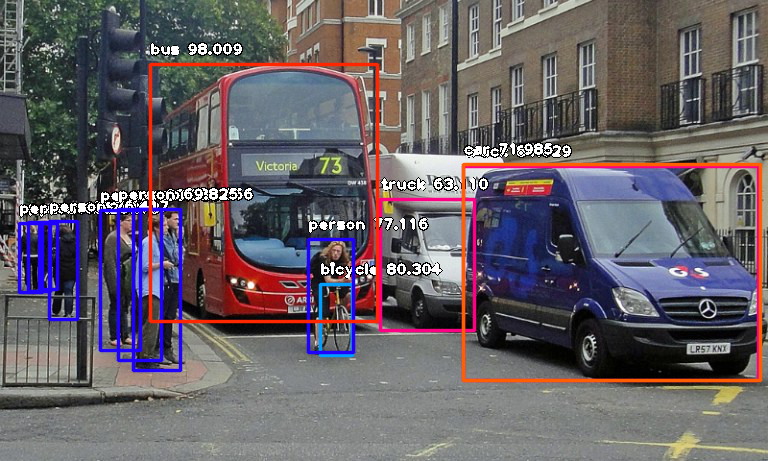
\includegraphics[width=11cm]{Obrazy/rozpoznawanieObiektow.jpeg}
        \caption{Przykład rozpoznawania obiektów na zdjęciu ulicy.~\cite{rozpoznawanieObiektow}}
        \label{fig.rozpoznawanieObiektow}
    \end{figure}

    Można znaleźć wiele witryn internetowych, które udostępniają interfejsy programistyczne umożliwiające zaimplementowanie
    rozpoznawania wieku z obrazu.
    Istnieją algorytmy przetwarzania obrazu, które oprócz wieku wyznaczają z pewnym prawdopodobieństwem płeć danej osoby.
    Oprócz płci mogą one także wyznaczyć mine oraz czy dana osoba nosi okulary.

    Z weryfikacją wieku danej osoby można się spotkać przed wejściem do niektórych miejsc, tj.
    klub nocny.
    Większość osób
    musi okazać ważny dowód osobisty,
    co generuje duże kolejki do wejścia.
    Aplikacje analizujące wiek na podstawie obrazu twarzy z kamery przed wejściem
    do takich miejsc znacząco usprawniłyby weryfikację wieku.
    Rozpoznawanie wieku może być wykorzystywane przy analizie średniego wieku ludzi w jakimś miejscu np.
    podczas demonstracji.

    Wiele gier posiada treści nieodpowiednie dla młodszych użytkowników.
    Możliwe jest stosowanie technologii wykrywania
    wieku użytkownika przed udostępnieniem mu treści, która wymaga odpowiedniego wieku.

    Można znaleźć o wiele więcej potencjalnych zastosowań przetwarzania obrazu oraz rozpoznawania wieku na podstawie
    tekstury (obrazu) twarzy.
    Z biegiem lat z pewnością będzie można zauważyć dalszy rozwój tej dziedziny, która
    opiera się w głównej mierze na sztucznej inteligencji~\cite{computerVision}.
    %275 wyrazow

    %    \section{Cel i zakres pracy}
    %    Celem pracy magisterskiej jest stworzenie prostego programu do rozpoznawania wieku na podstawie tekstury twarzy.
    %
    %    Zakres pracy obejmuje:
    %    \begin{itemize}
    %        \item Wybór bazowej metody wyznaczania wieku
    %        \item Stworzenie kilku modyfikacji bazowej metody
    %        \item Opis algorytmów każdej z metod wyznaczania wieku
    %        \item Porównanie wszystkich metod i wybór najlepszej
    %    \end{itemize}
    %
    %    \chapter{Przegląd metod wyznaczania wieku}
    %    \section{Metoda a}
    %    \section{Metoda b}
    %    \section{Metoda wrinkle feature}

    \chapter{Metoda bazowa - wrinkle feature}\label{ch:metoda-bazowa---wrinkle-feature}

    Istnieje wiele metod wyznaczania wieku z obrazu twarzy.
    W literaturze spotkano rozwiązania, w których wyznaczany
    jest konkretny
    wiek osoby przez algorytm lub przedział wiekowy.
    Jedna z pierwszych metod szacowania wieku opierała się na wyznaczaniu proporcji twarzy, a następnie na detekcji i
    interpretacji zmarszczek.
    Była ona w stanie ze stu procentową poprawnością wyznaczyć czy dana osoba jest osobą
    dorosłą lub
    dzieckiem~\cite{kwonLobo}.

    W kolejnych latach algorytmy i techniki szacowania wieku były udoskonalane.
    Badano wpływ starzenia się osób na
    wygląd skóry.
    Oprócz naturalnych zmian skóry pod wpływem starzenia się skóry należało uwzględnić także inne
    czynniki.
    Takimi czynnikami są min.
    płeć, poziom stresu, ekspozycja na działanie środowiska zewnętrznego.
    Powyższe metody zastosowano w pracy ,,Toward automatic simulation
    of aging effects on face images'' autorstwa A. Lanitis, Ch. J. Taylor oraz T. F. Cootes~\cite{lanitisTaylor}.
    Należy dodać, że w powyższej pracy stosowano trenowanie zbioru zdjęć.
    Trenowanie polega na wykryciu relacji pewnych cech twarzy do wieku osób.

    W kolejnych latach pojawiło się podejście porównywania cech twarzy tej samej osoby w różnym wieku.
    Różnice w powyższych cechach posłużyły do zbudowania statystyki zmian cech twarzy wraz ze starzeniem się.
    Powyższe podejście zostało zaprezentowane w pracy ,,Face verification across age progression''
    autorstwa N. Ramanathan oraz R. Chellappa~\cite{ramanthanChelappa}.

    Rozwinięciem tego pomysłu była praca ,,Automatic age estimation based
    on facial aging patterns'' autorstwa X. Geng, Z. Zhou i K. Smith-Miles~\cite{gengZhou}.
    W tej pracy porównywano sekwencje wielu zdjęć twarzy jednej osoby.
    Zdjęcia przestawiały twarz w różnym wieku.
    Powyższe badania pozwoliły na zbudowanie wzorca starzenia się twarzy.

    Praca ,,A new algorithm for age recognition
    from facial images'' autorstwa M.M. \ Dehshibi oraz A. Bastanfard~\cite{dehshibiBastard} przy szacowaniu wieku
    analizuje proporcje twarzy oraz ilość zmarszczek.

    Praca ,,Age Estimation from Face Images: Challenging
    Problem for Audience Measurement Systems'' autorstwa
    Vladimira Khryashcheva, Alexandra Ganina, Olgi Stepanovej oraz
    Antona Lebedeva podsumowała techniki szacowania wieku~\cite{khryashchevGanin}.
    Z podsumowania wynikło, że najczęściej stosuje się do wyodrębniania cech z twarzy BIF,
    czyli biologically inspired features.
    Powyższa metoda została zaprezentowana w książce ,,Human Age Estimation Using Bio-inspired Features''
    autorstwa Guodong Guo i in.
    Mniej popularne metody analizujące cechy twarzy to filtry Gabora oraz LBP- local binary patterns.


    Metoda bazowa została opisana w artykule ,,Age Estimation from Face Image using Wrinkle Features''
    ~\cite{wrinkleFeatures}.
    Wykrywanie wieku dzieli się na kilka faz.
    Na początku należy wykryć twarz.
    Zastosowany algorytm wykrywania został
    opisany w sekcji~\ref{sec:metodaWykrywaniaTwarzy}
    Następnie należy wyznaczyć strefy zmarszczkowe na twarzy.
    W artykule~\cite{wrinkleFeatures} udowodniono,
    że istnieje kilka konkretnych stref, w których następuje znacząca zmiana ilości zmarszczek wraz z wiekiem.
    Powyższe strefy zostały wymienione w sekcji~\ref{sec:wyznaczanieStref}.
    Sekcja~\ref{sec:wykrywanieZmarszczek} przedstawia technikę wykrywania zmarszczek znajdujących się w strefach.
    Wykryte zmarszczki
    pozwalają na obliczenie wrinkle feature dla danej twarzy, zgodnie z opisem w sekcji~\ref{sec:wyliczanieWrinkleFeature}.
    W tym miejscu kończy się faza wyznaczania wrinkle feature dla danej osoby (Rysunek~\ref{fig.faza1Algorytmu}).
    Kolejna faza
    jest potrzebna do
    znalezienia relacji pomiędzy wrinkle feature a wiekiem.
    Do tego celu należy zastosować algorytm trenujący, który
    został opisany w sekcji~\ref{sec:algorytmTrenowania}.
    Wynikiem algorytmu trenującego jest zbiór danych, który
    należy pogrupować, tak jak to opisano w sekcji~\ref{sec:grupowanieDanych}.
    Ostatnią fazą algorytmu jest wykrywanie wieku
    na podstawie wyników działania FCM - sekcja~\ref{sec:wyznaczanieWieku} (Rysunek~\ref{fig.faza2Algorytmu}).

    \begin{figure}[h]
        \centering
        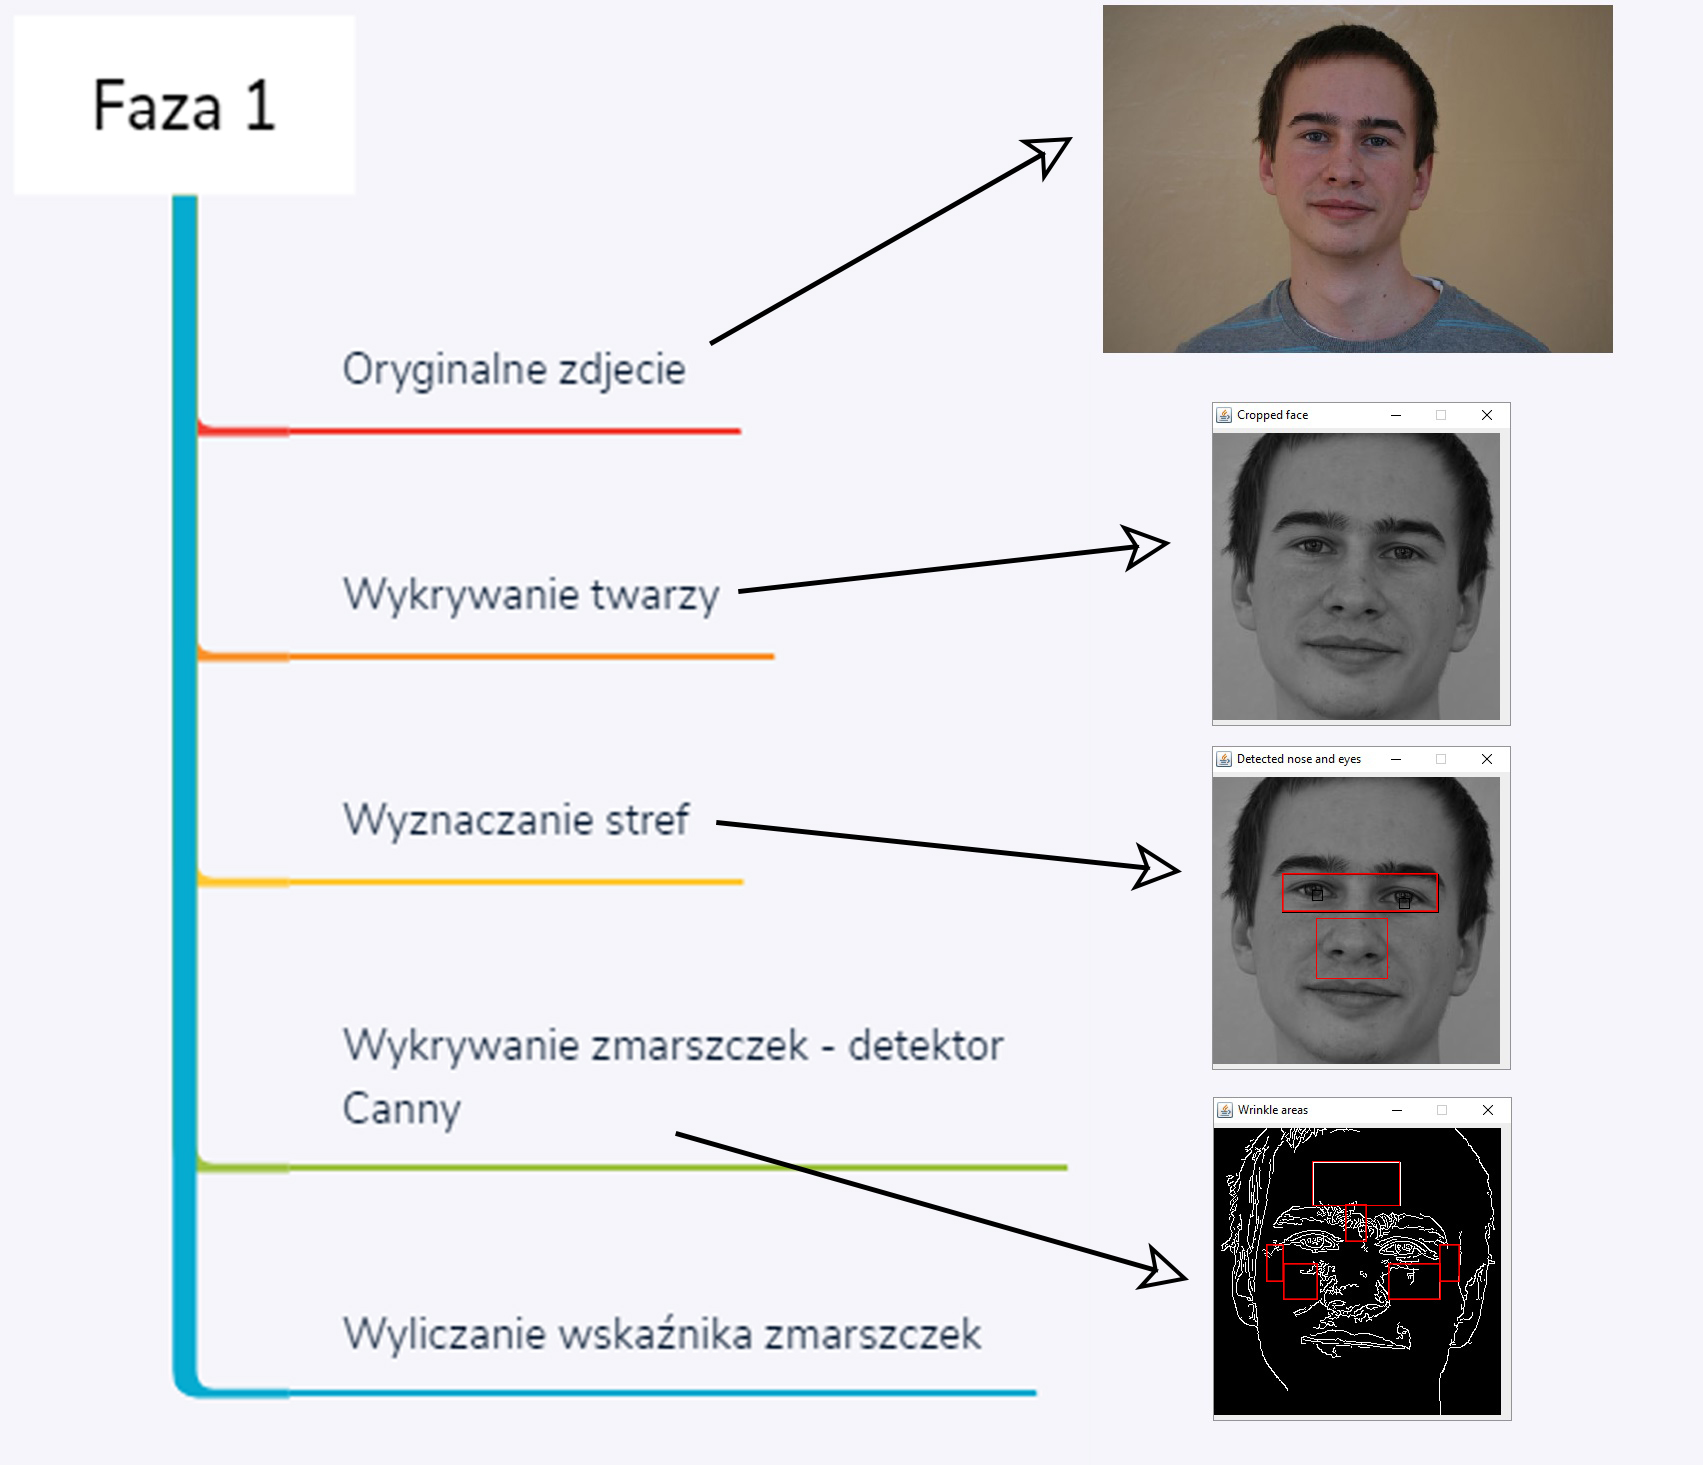
\includegraphics[width=8cm]{Obrazy/Faza1.jpg}
        \caption{Faza 1 algorytmu}
        \label{fig.faza1Algorytmu}
    \end{figure}

    \begin{figure}[h]
        \centering
        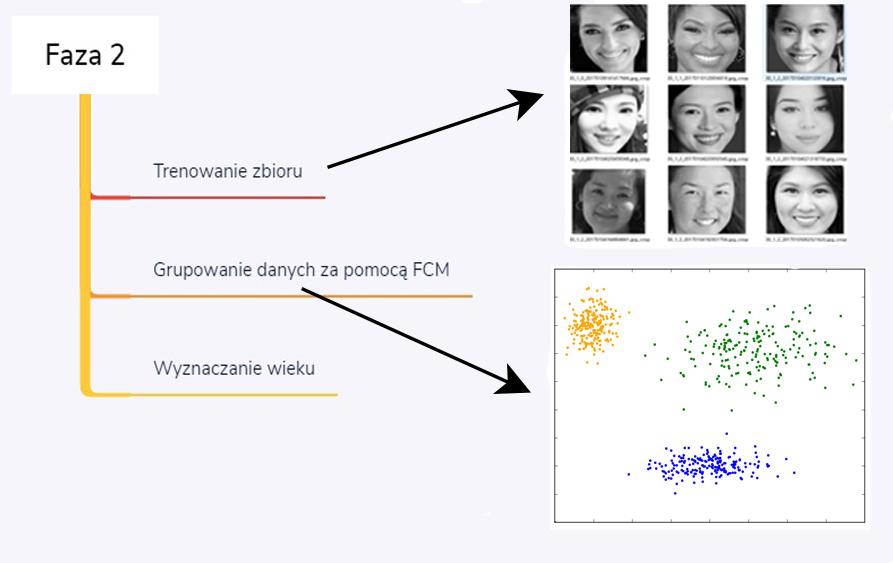
\includegraphics[width=8cm]{Obrazy/Faza2.jpg}
        \caption{Faza 2 algorytmu}
        \label{fig.faza2Algorytmu}
    \end{figure}

    \section{Metoda wykrywania twarzy}\label{sec:metodaWykrywaniaTwarzy}
    W literaturze można odnaleźć wiele metod wykrywania twarzy.
    Istnieje kilka podejść aby skutecznie wykrywać twarz na danym obrazie~\cite{mehdiRizvi}:
    %       https://www.researchgate.net/publication/257338580_A_Review_on_Face_Detection_Methods
    %     Knowledge-based methods: These rule-based methods encode human knowledge
    %    of what constitutes a typical face. Usually, the rules capture the relationships
    %    between facial features. These methods are designed mainly for face localization.
    %     Feature invariant approaches: These algorithms aim to find structural features that
    %    exist even when the pose, viewpoint, or lighting conditions vary, and then use these
    %    to locate faces. These methods are designed mainly for face localization.
    %     Template matching methods: Several standard patterns of a face are stored to
    %    describe the face as a whole or the facial features separately. The correlations
    %    between an input image and the stored patterns are computed for detection. These
    %    methods have been used for both face localization and detection.
    %     Appearance-based methods: In contrast to template matching, the models (or
    %    templates) are learned from a set of training images which should capture the
    %    representative variability of facial appearance. These learned models are then used
    %    for detection. These methods are designed mainly for face detection.

    \begin{itemize}
        \item metoda oparta na nauce
        \item metoda niezmienności cech
        \item metoda dopasowania szablonu twarzy
        \item metoda bazująca na wyglądzie
    \end{itemize}
    Metoda oparta na nauce kieruje się wiedzą na temat wyglądu twarzy, a
    bardziej precyzyjnie chodzi o charakterystyczne cechy,
    dzięki którym na zdjęciu można wyodrębnić obszar twarzy.
    Mowa tutaj o cechach takich jak kształt twarzy, kolor, miejsca o różnej jasności czy specyficzne krawędzie tworzone np przez
    usta.

    W metodzie niezmienności cech wyszukuje się takie strukturalne cechy twarzy, które są widoczne w każdych warunkach
    oświetleniowych.
    Ponadto te cechy są widoczne bez względu na punkt widzenia, nawet jeśli twarz jest widoczna
    z profilu czy przechylona pod kątem.

    Z kolei metoda dopasowania szablonu twarzy wykorzystuje kilka standardowych wzorów opisujących twarz.
    Na wejściu algorytmu obraz jest porównywany z tymi wzorami, a
    na wyjściu dostajemy informację, w jakim stopniu obraz jest dopasowany do szablonu twarzy.

    Ideą metody bazującej na wyglądzie jest trenowanie dużego zbioru obrazów twarzy, tak aby wychwycić zmienność cech
    twarzy.
    Tak wytrenowany model jest później wykorzystywany do wykrywania twarzy.


    Ponadto w procesie ekstrakcji twarzy z obrazu istnieje wiele problemów~\cite{mehdiRizvi}.
    %       https://www.researchgate.net/publication/257338580_A_Review_on_Face_Detection_Methods
    %    Pose: The images of a face vary due to the relative camera-face pose (frontal, 45
    %    degree, profile, upside down), and some facial features such as an eye or the nose
    %    may become partially or wholly occluded.
    %     Presence or absence of structural components: Facial features such as beards,
    %    mustaches, and glasses may or may not be present and there is a great deal of
    %    variability among these components including shape, color, and size.
    %     Facial expression: The appearance of faces is directly affected by a person’s facial
    %    expression.
    %     Occlusion: Faces may be partially occluded by other objects. In an image with a
    %    group of people, some faces may partially occlude other faces.
    %     Image orientation: Face images directly vary for different rotations about the
    %    camera’s optical axis.
    %     Imaging conditions: When the image is formed, factors such as lighting (spectra,
    %    source distribution and intensity) and camera characteristics (sensor response,
    %    lenses) affect the appearance of a face.
    %    Każda z nich wyodrębnia z obrazu pewne cechy, które
    %    mogą wskazywać, że na danym obszarze obrazu znajduje się twarz.

    Jednym z problemów jest nieodpowiednia poza.
    Wiąże się to z różnymi ustawieniami twarzy wobec aparatu fotograficznego lub kamery.
    Twarz może być nachylona, przechylona lub odchylona.
    Inaczej mówiąc może mieć różne położenie w trzech wymiarach, a
    niektóre części twarzy lub jej cechy mogą zostać przysłonięte.
    Im mniej cech widocznych na twarzy, tym mniej danych, które algorytm może z niej wyodrębnić, a
    im mniej danych, którymi algorytm operuje, tym mniejsze prawdopodobieństwo prawidłowego wykrycia twarzy.

    Niektóre twarze mogą zawierać pewne wyróżniające je cechy takie jak broda, blizny czy okulary.
    Różnorodność tych cech także wpływa na efektywność wykrywania twarzy.

    Ilość zmarszczeń na twarzy jest zmienna, w zależności od wyrazu mimicznego.
    Przy różnych minach zmienia się kształt ust, a czasem pojawiają się ostre krawędzie wynikające z pracy mięśni twarzowych.
    Widoczne mogą być różne pofałdowania skóry.

    Zdarza się, że twarz zostaje częściowo przysłonięta przez jakiś inny obiekt.
    Na przykład na zdjęciu,
    które obejmuje grupę wielu osób, część danej twarzy może być przysłonięta przez inną twarz.
    Takie przysłonięcie przez inny obiekt wiąże się z utratą informacji o części twarzy, co zmniejsza prawdopodobieństwo
    prawidłowego jej wykrycia.

    Kolejnym istotnym elementem jest oświetlenie twarzy.
    Gdy twarz oświetlona jest tzw. twardym światłem, występują na
    niej cienie i światła określane jako ostre (Sekcja~\ref{fig.oswietlenieTwarzy}).
    \begin{figure}
        \centering
        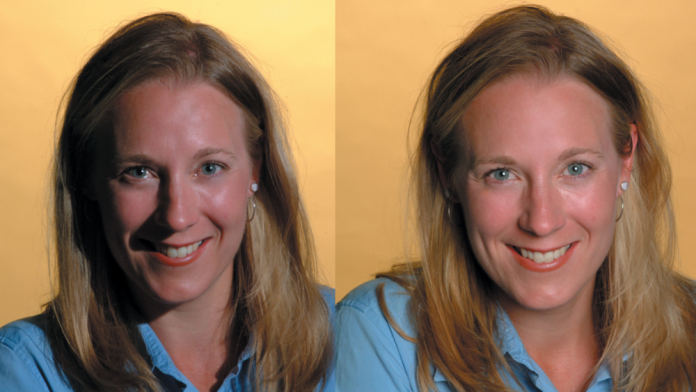
\includegraphics[width=12cm]{Obrazy/oswietlenieTwarzy.jpg}
        \caption{Przykład twarzy oświetlonej twardym (twarz po lewej) oraz miękkim światłem.~\cite{oswietlenieTwarzy}}
        \label{fig.oswietlenieTwarzy}
    \end{figure}
    W tym przypadku ryzyko utraty szczegółów oświetlanej twarzy jest większe.
    Kiedy twarz jest skierowana na wprost słońca, z dużym
    prawdopodobieństwem można stwierdzić, że zostanie oświetlona twardym światłem.
    Z kolei miękkie światło jest generowane na przykład przez zachmurzone niebo.
    Istotne jest także źródło światła, które
    może być punktowe lub rozproszone.
    Przy punktowym źródle światła cała twarz jest
    okryta jednolitym cieniem, którego intensywność zależy od "twardości" światła.
    Natomiast przy świetle rozproszonym intensywność cieni jest mniejsza.

    Na Rys~\ref{fig.technikiWykrywaniaTwarzy} przedstawione są różne techniki wykrywania twarzy.
    \begin{figure}
        \centering
        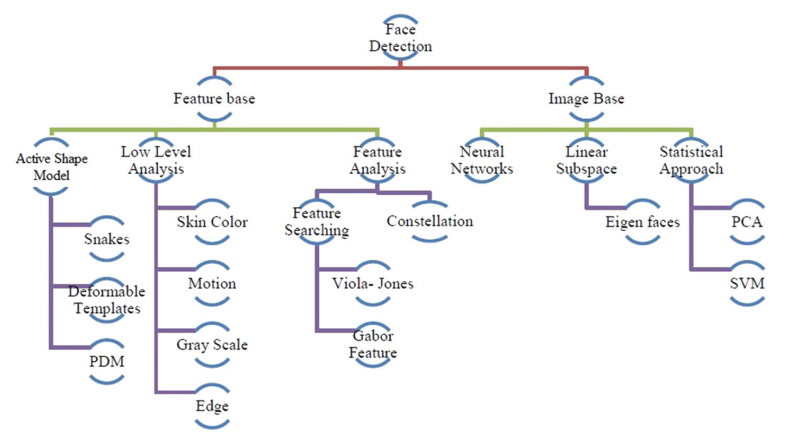
\includegraphics[width=15cm]{Obrazy/technikiWykrywaniaTwarzy.jpg}
        \caption{Różne techniki wykrywania twarzy.~\cite{faceDetectionTechniques}}
        \label{fig.technikiWykrywaniaTwarzy}
    \end{figure}
    %    https://sci-hub.tw/10.1007/s10462-018-9650-2

    %    Wyodrębnianie lub ekstrakcja cech polega na przekształceniu obrazu do zbioru zmiennych, które
    %    zostaną później użyte w wykrywaniu obiektu lub obiektów na obrazie.

    Jak widać metod wykrywania twarzy jest sporo.
    Omówienie każdej z nich zajęłoby dużo czasu.
    Poniżej zostaną przytoczone dwie metody wykrywania twarzy.
    Dodatkowo zostanie omówiona metoda, która posłużyła do wykrywania twarzy w niniejszej pracy.

    %https://sci-hub.tw/10.1016/S0031-3203(00)00134-5
    W pracy ,,An efficient algorithm for human face detection and facial
    feature extraction under different conditions''~\cite{wongLamSiu}
    przedstawiono opisaną w skrócie poniżej technikę wykrywania twarzy.
    W pierwszym etapie procesu obszary, gdzie może znajdować się ludzkie oko,
    są wykrywane przez przeprowadzenie testów na zacienionych rejonach obrazu.
    Pary takich obszarów wyodrębnia się na podstawie algorytmu genetycznego,
    aby następnie wyznaczyć możliwy obszar twarzy.
    Dla każdego obszaru mierzy się wartość dopasowania na podstawie jego projekcji na wektory własne,
    tzw. eigenfaces.
    Aby wiarygodność wykrywania była wyższa,
    każdy możliwy obszar twarzy normalizuje się pod kątem oświetlenia.
    Proces ten powtarza się pewną ilość razy,
    a następnie do dalszej weryfikacji są wybierane możliwe obszary twarzy o wysokiej wartości dopasowania.
    Na tym etapie mierzy się symetrię twarzy oraz sprawdza się,
    czy na każdym wybranym obszarze istnieją rysy twarzy.
    Rysy określa się przez ewaluację rzeźby topograficznej - wystających i wklęsłych elementów
    różnych regionów obszaru twarzy, poddanego uprzednio normalizacji.
    Algorytm jest w stanie wykryć także obszar twarzy, gdy głowa jest przechylona

    %todo Druga metoda wykrywania twarzy z https://www.researchgate.net/publication/334770252_An_Accurate_System_for_Face_Detection_and_Recognition
    %todo https://sci-hub.tw/10.1007/s10462-018-9650-2
    W roku 1997 w pracy pt. ,,Vision for man-machine interaction'' opisano metodę wykrywania twarzy bazującą na
    wykrywaniu cechy jaką jest kolor skóry~\cite{clowleyCoutaz}.
    Kolor skóry jest najbardziej widoczną cechą twarzy zarówno dla człowieka jak i dla maszyny.
    Ponadto kolor jest przetwarzany znacznie szybciej od innych cech.
    Przy dobrych warunkach oświetleniowych ustawienie twarzy nie ma wpływu na skuteczność wykrywalności twarzy
    opisywaną metodą.
    Każda metoda wykrywania twarzy posiada wady.
    Jedną z tych wad jest problem wykrywalności twarzy przy nierównomiernym oświetleniu.
    Problem pojawia się także, gdy na obrazie widoczny jest obszar skóry z poza twarzy np. z rąk.
    Warto zaznaczyć, że kolor twarzy na obrazie jest zależny od względnego kierunku oświetlenia.
    Obszar twarzy w omawianym algorytmie jest wykrywany poprzez normalizacje histogramu kolorów.
    Normalizacja jest potrzebna do redukcji wpływu luminancji na kolor.

    %todo trzecia metoda  - wstep do Haar Cascade https://drive.google.com/file/d/1nJ9S3HtuuFY6O1FLdIjRWSzWUFwZ_fuJ/view?usp=sharing
    Algorytm Haar Cascade jest najpopularniejszym algorytmem do wykrywania twarzy w bibliotece OpenCV. Właśnie ta
    biblioteka była jednym z niezbędnym elementów programu przy wykrywaniu wieku z tekstury twarzy.
    W związku z powyższym w wykrywaniu twarzy zastosowano algorytm Haar Cascade.
    Omawiany algorytm został zaprezentowany w książce ,,Rapid Object Detection using a Boosted Cascade of Simple
    Features'' w 2001 i składa się z trzech faz~\cite{violaJones}.
    W pierwszej obraz wejściowy przekształcany jest na obraz scałkowany.
    Następnie wykorzystywany jest algorytm do boostingu, który zmniejsza ilość klasyfikatorów tylko do tych
    najbardziej istotnych.
    W ostatniej fazie klasyfikatory łączone są w kaskady w celu przyspieszenia procesu wykrywania twarzy.
    Znaczna większość metod wykrywania obiektów na obrazie (w tym twarzy) wymaga wstępnego przekształcenia obrazu do
    skali szarości.

    %    https://towardsdatascience.com/face-recognition-with-opencv-haar-cascade-a289b6ff042a
    %    przez kogo został zaproponowany...
    %    byc moze cos o funkcji kaskadowej
    %    o tym ze OpenCv zawiera wytrenowane algorytmy Haar Cascade ktore wykrywaja ryj, oczy, usta itp
    %    wkleic obrazek z rodzajami filtrow
    %    jak dziala ten filtr
    %    przyklad na gebie emmy watson moze...
    %cosik tam jeszcze

    %    opisac jak dokladnie zaimplementowano to u nas
    %    przejscie na skale szarosci podczas wykrywania... czym ona jest?...
    \subsection{Konwersja do skali szarości oraz przestrzenie barw}\label{subsec:konwersja-do-skali-szarości-oraz-przestrzenie-barw}
    %todo https://sci-hub.tw/10.1007/s10462-018-9650-2
    Każdy piksel w trybie kolorowym ma określoną reprezentację barwy z określonego modelu.
    Najczęściej są to 3 lub 4 wartości~\cite{przestrzenieKolorow}.
    Pierwszą przestrzenią barw była CIEXYZ. Została ona stworzona w 1931 przez
    Międzynarodowa Komisja ds. Oświetlenia (International Commission on Illumination).
    Przestrzeń barw CIEXYZ została specjalnie stworzona, by odtworzyć sposób postrzegania barw przez ludzkie oko.
    Barwa jest opisywana w trzech współrzędnych trójchromatycznych X,Y,Z.
    Powyższe współrzędne są zależne od składowych - sprawności wizualnych czopków.
    Czopki to światłoczułe receptory siatkówki ludzkiego oka~\cite{przestrzenieKolorow}.
    Współrzędne X,Y,Z wyliczane są na podstawie trzech podstawowych barw R (czerwonej),
    G (zielonej) i B (niebieskiej).
    Współrzędne XYZ są często reprezentowane przez luminancję Y oraz współrzędne x, y chromatyczności.
    Wyliczanie współrzędnych x, y przedstawiono na wzorach~\ref{wzor.chromX} oraz~\ref{wzor.chromY}.
    \large
    \begin{equation}
        x = \frac{X}{X+Y+Z}
        \label{wzor.chromX}
    \end{equation}
    \normalsize

    \large
    \begin{equation}
        y = \frac{Y}{X+Y+Z}
        \label{wzor.chromY}
    \end{equation}
    \normalsize

    Na Rysunku~\ref{fig.CIEXYZ} przedstawiono diagram chromatyczności reprezentujący przestrzeń barw CIEXYZ.

    \begin{figure}
        \centering
        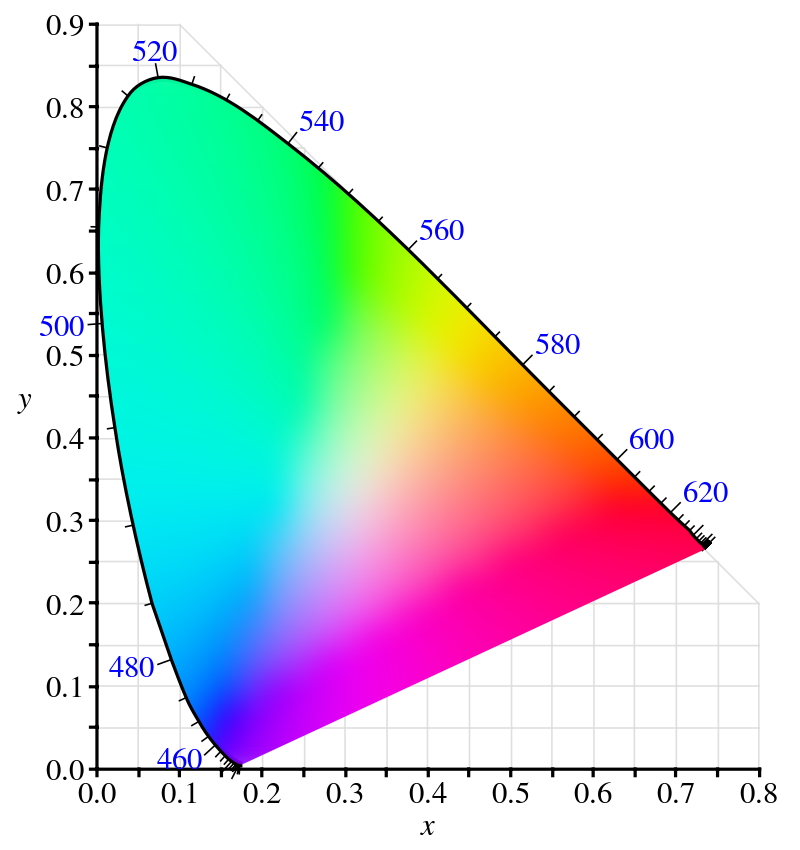
\includegraphics[width=6cm]{Obrazy/CIEXYZ.jpg}
        \caption{Przykład rozpoznawania obiektów na zdjęciu ulicy.~\cite{diagramCIEXYZ}}
        \label{fig.CIEXYZ}
    \end{figure}

    Kolory mogą byc także odwzorowane przez przestrzeń barw CMYK.
    Skrót CMYK oznacza odpowiednio:
    \begin{itemize}
        \item Cyan - odcień niebieskiego
        \item Magenta - kolor karmazynowy
        \item Yellow - kolor żółty
        \item K - key colour - kolor czarny
    \end{itemize}
    Barwa wynikowa powstaje poprzez mieszanie trzech kolorów - niebieskiego, karmazynowego oraz żółtego.
    Mieszanie zachodzi według zasady syntezy subtraktywnej~\cite{przestrzenieKolorow}.
    Synteza subtraktywna polega na mieszaniu kolorów przez odejmowanie promieniowań widzialnych różnych długości.
    Przykładem syntezy subtraktywnej jest np. mieszanie farb o różnych kolorach.

    Najczęściej barwy są reprezentowane przez przestrzeń barw RGB~\cite{przestrzenieKolorow}.
    Przestrzeń kolorów RGB składa się z trzech kanałów~\cite{kolory}:

    \begin{itemize}
        \item R - czerwonego (z angielskiego Red)
        \item G - zielonego (z angielskiego Green)
        \item B - niebieskiego (z angielskiego Blue)
    \end{itemize}
    Barwy mieszane są poprzez syntezę addytywną .
    W przeciwieństwie do syntezy subtraktywnej barwa wynikowa powstaje poprzez sumowanie wiązek światła widzialnego o
    różnych długościach~\cite{przestrzenieKolorow}.
    Każdy piksel opisany za pomocą przestrzenie barw RGB ma trzy 8-bitowe wartości reprezentujący każdy kanał.
    Spotykane
    są 12- lub 16-bitowe reprezentacje kanałów, jednak 8-bitowa jest najpopularniejsza.
    Dla 8-bitowych kanałów
    wartość ,,0''
    danego kanału oznacza brak jasności, natomiast ,,255'' maksymalną jasność.
    Poprzez mieszanie jasności tych trzech kanałów
    można uzyskać szerokie spektrum barw (Rysunek~\ref{fig.mieszanieKolorow}).

    \begin{figure}
        \centering
        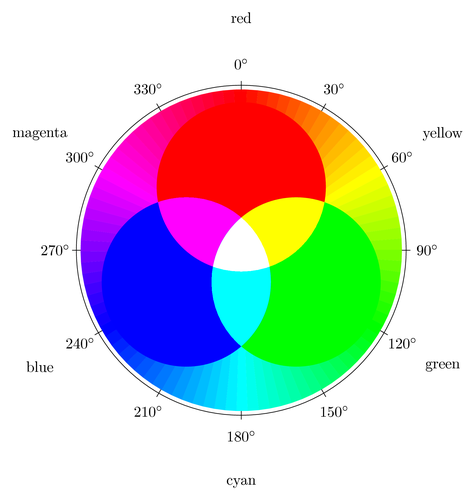
\includegraphics[width=7cm]{Obrazy/mieszanieKolorow.jpg}
        \caption{Mieszanie kanałów RGB~\cite{colorMixing}.}
        \label{fig.mieszanieKolorow}
    \end{figure}

    Przykładowo kolor o reprezentacji R=153 G=217 B=234 przedstawiono na Rysunku~\ref{fig.mieszanieKolorowBlekitny}

    \begin{figure}
        \centering
        
\includegraphics[width=2cm]{Obrazy/blekitny.jpg}
        \caption{Kolor R=153 G=217 B=234.}
        \label{fig.mieszanieKolorowBlekitny}
    \end{figure}

    Kolor (Rysunek~\ref{fig.mieszanieKolorowBlekitny}) może być też reprezentowany w kodzie szesnastkowym \#99D9EA.
    Każda
    wartość heksadecymalna odpowiada kolejno kanałowi R, G, B.

    Obraz może też być przedstawiony stosując odcienie jednej barwy.
    Taka obraz nazywa się obrazem monochromatycznym.
    Najczęściej stosowaną barwą w takich obrazach jest szarość~\cite{przestrzenieKolorow}.

    Istnieją 3 metody konwersji obrazu z przestrzeni RGB na monochromatyczny~\cite{colorMixing}.
    \begin{itemize}
        \item największej jasności
        \item średnia
        \item luminancji
    \end{itemize}
    Metoda największej jasności konwertuje na skalę szarości wg wzoru\ref{wzor.najwiekszaJasnosc}.

    \large
    \begin{equation}
        \frac{(max(R, G, B) + min(R, G, B))}{2}
        \label{wzor.najwiekszaJasnosc}
    \end{equation}
    \normalsize
    Metoda średnia bazuje na wzorze~\ref{wzor.metodaSrednia}, natomiast metodę luminancji ilustruje wzór~\ref{wzor.metodaLuminancji}.

    \large
    \begin{equation}
        \frac{(R + G + B)}{3}
        \label{wzor.metodaSrednia}
    \end{equation}
    \normalsize

    \large
    \begin{equation}
        0.21 R + 0.72 G + 0.07 B
        \label{wzor.metodaLuminancji}
    \end{equation}
    \normalsize

    W niniejszej pracy zastosowano konwersję za pomocą metody średniej.
    \subsection{Algorytm Haar Cascade}\label{subsec:algorytm-haar-cascade}

    Haar Cascade jest algorytmem służącym do wykrywania obiektów na obrazach.
    Został stworzony przez Paula Viola oraz Michaela Jonesa w 2001 roku~\cite{violaJones}.

    Opiera się na zbudowaniu kaskadowej funkcji za pomocą trenowania wielu zdjęć.
    Zdjęcia są dzielone na
    dwie kategorie - pozytywne oraz negatywne.
    Na zdjęciach klasyfikowanych jako pozytywne istnieje obiekt, który ma zostać wykryty, natomiast
    na zdjęciach negatywnych nie ma tego obiektu.

    Ekstrakcja cech w algorytmie Violi i Jonesa jest realizowana przez filtry Haara.
    Są to prostokątne okienka
    nakładane na obraz, które analizują jasność pikseli (Rysunek~\ref{fig.haarRectangles}).
    \begin{figure}
        \centering
        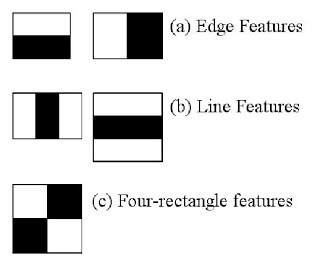
\includegraphics[width=7cm]{Obrazy/Haar_filter_rectangles.jpg}
        \caption{Filtr Haara a) krawędziowy b) liniowy c) szachownica~\cite{haar}}
        \label{fig.haarRectangles}
    \end{figure}

    Przed zastosowaniem filtru Haara obraz musi zostać przekształcony do skali szarości
    W niniejszej pracy należało przekształcić każdy obraz z trybu kolorowego na monochromatyczny, co opisano w sekcji~\ref{subsec:konwersja-do-skali-szarości-oraz-przestrzenie-barw}.

    Każde okienko zawiera białe oraz czarne prostokąty.
    Wyznaczana jest suma jasności pikseli w obu rodzajach prostokątów, a
    następnie dla każdego okna obliczana jest różnica pomiędzy białymi a czarnymi.
    Opisywany algorytm ma zastosowanie w wykrywaniu krawędzi.
    Na granicy krawędzi istnieje różnica w jasności pikseli
    (Rysunek~\ref{fig.haarEmmaWatson}).

    \begin{figure}
        \centering
        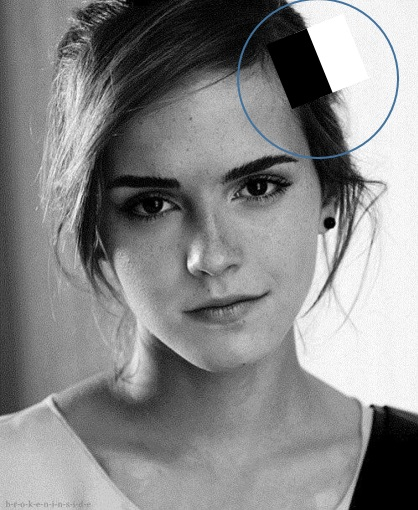
\includegraphics[width=6cm]{Obrazy/haarEmmaWatson.jpg}
        \caption{Filtr Haara nałożony na krawędź twarzy~\cite{haar}}
        \label{fig.haarEmmaWatson}
    \end{figure}

    W celu poprawy efektywności sumowania pikseli stosowane są
    rozwiązanie zwane w języku angielskim Summed-area table~\cite{violaJonesRealTimeOb}.Summed-area table jest również
    nazywana w literaturze Integral Image, czyli obrazem scałkowanym.
    Ideą obrazu scałkowanego jest,
    aby każdy obraz
    został
    przekształcony w
    tabelę, w której każdy element x,y tej tabeli odpowiada sumie jasności wszystkich pikseli według wzoru~\ref{wzor.summedAreaTable}.

    \large
    \begin{equation}
        I(x,y) = \sum_{{x}'\leq x \cap {y}'\leq y}^{} i({x}',{y}')
        \label{wzor.summedAreaTable}
    \end{equation}
    \normalsize
    gdzie I(x,y) jest wartością na pozycji x,y w tabeli(tabela obrazu scałkowanego), natomiast i(x,y) oznacza jasność piksela o
    współrzędnych x,y na obrazie.

    Na Rysunku~\ref{fig.przedCalkowaniem} przedstawiona jest tabela prezentująca jasność pikseli przed
    zastosowaniem całkowania obrazu.
    \begin{figure}
        \centering
        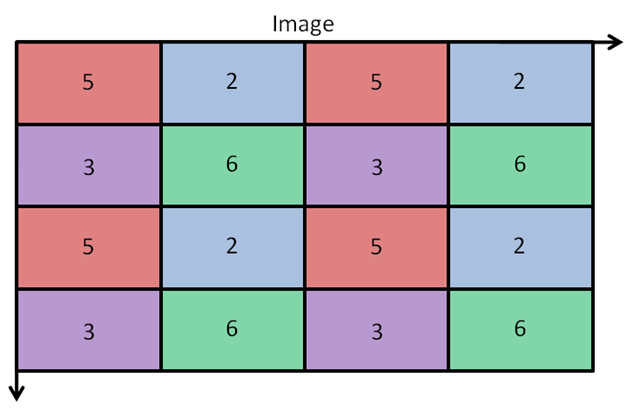
\includegraphics[width=6cm]{Obrazy/przedCalkowaniem.jpg}
        \caption{Tabela jasności poszczególnych pikseli przed zastosowaniem całkowania~\cite{integralImages}}
        \label{fig.przedCalkowaniem}
    \end{figure}

    Po całkowaniu otrzymujemy tabelę podobną do przedstawionej na Rysunku~\ref{fig.poCalkowaniu}.
    \begin{figure}
        \centering
        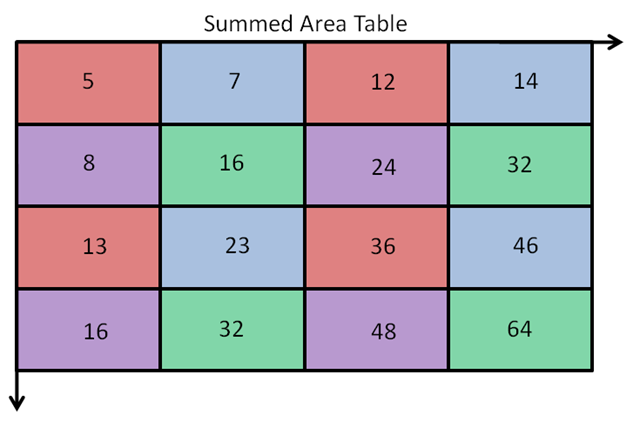
\includegraphics[width=6cm]{Obrazy/poCalkowaniu.jpg}
        \caption{Filtr Haara nałożony na krawędź twarzy~\cite{integralImages}}
        \label{fig.poCalkowaniu}
    \end{figure}

    Sumowanie przykładowego okna (Rysunek~\ref{fig.sumowanieOkna}) wymaga czterech operacji (Wzór~\ref{wzor
    .windowsSum}).
    \begin{figure}
        \centering
        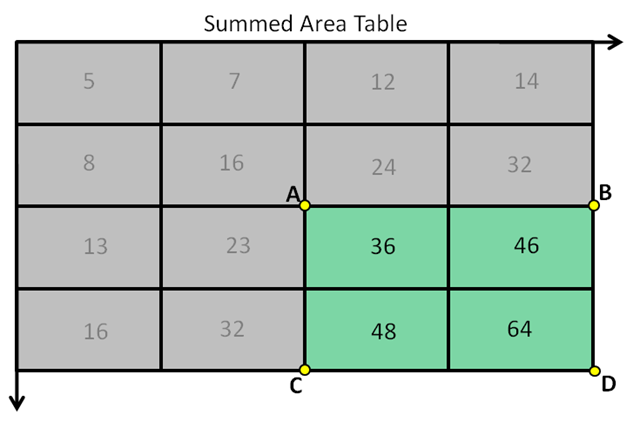
\includegraphics[width=6cm]{Obrazy/sumowanieOkna.jpg}
        \caption{Sumowanie okna~\cite{integralImages}}
        \label{fig.sumowanieOkna}
    \end{figure}


    \large
    \begin{equation}
        \sum_{x_0\leq x \leq x_1\cap {y}\leq y \leq y_1}^{} i(x,y) = I(D) + I(A) - I(B) - I(C)
        \label{wzor.windowsSum}
    \end{equation}
    \normalsize
    gdzie lewa część równania oznacza sumę jasności pikseli
    zaznaczonego okna tj.
    na Rysunku~\ref{fig.sumowanieOkna}, I(A) - wartość scałkowanego obrazu przy punkcie A
    (analogicznie I(B), I(C), I(D)) - (Rysunek~\ref{fig.sumowanieOkna}).

    W związku z powyższym obliczenie wartości dla krawędziowego filtru Haara wymaga obliczenia różnicy dwóch sum, zatem konieczne jest wykonanie
    ośmiu operacji.
    Reprezentacja obrazu za pomocą obrazu scałkowanego znacznie zwiększa efektywność obliczania wartości w filtrze
    Haara.


    Liczba cech wykrywanych w danym zdjęciu za
    pomocą filtru Haara jest znacznie większa od liczby pikseli na obrazie~\cite{violaJones}.
    Dla obrazu o wymiarach 384x288 pikseli liczba cech wynosi ponad 180000.
    Autorzy algorytmu stwierdzili, że dla zwiększenia jego szybkości należy wybrać małą grupę cech,
    które razem mogą stworzyć jeden efektywny klasyfikator obiektu.
    W celu wyodrębnienia tych istotnych cech zastosowano algorytm Adaboost, który został opisany poniżej.

    Zbiór n obrazów do trenowania można oznaczyć tak jak we wzorze~\ref{wzor.zbiorTrenujacy}:
    \large
    \begin{equation}
        (x_1, y_1), (x_2, y_2), \ldots, (x_n, y_n)
        \label{wzor.zbiorTrenujacy}
    \end{equation}
    \normalsize

    oznacza, że obraz jest odpowiednio negatywny lub pozytywny.
    Następnym krokiem jest inicjalizacja wag (Wzór~\ref{wzor.wagi}).

    \large
    \begin{equation}
        w_{1,i} = \frac{1}{2m}, \frac{1}{2l}
        \label{wzor.wagi}
    \end{equation}
    \normalsize
    odpowiednio dla $y_i = 0, 1$
    , gdzie m, l oznacza odpowiednio liczbę negatywnych oraz pozytywnych zdjęć.
    Następnie
    Dla t = 1, \ldots, T:

    1. Normalizowane są wagi (Wzór~\ref{wzor.adaboost1}):
    \large
    \begin{equation}
        w_{t,i} = \frac{w_{t,i}}{\sum_{j=1}^{n}w_{t,j}}
        \label{wzor.adaboost1}
    \end{equation}
    \normalsize
    $w_{t}$ jest rozkładem prawdopodobieństwa

    2. Dla każdej cechy j, trenowany jest klasyfikator $h_{j}$, który używa tylko jednej cechy wyliczonej z filtru Haara.
    Błąd jest liczony następująco (Wzór~\ref{wzor.adaboost2}):
    \large
    \begin{equation}
        w_{t}, \epsilon_{j} = \sum_{i}^{}w_{i} \abs{h_{j}(x_{i}) - y_{i}}
        \label{wzor.adaboost2}
    \end{equation}
    \normalsize

    3. Wybierany jest klasyfikator $h_{t}$ z najmniejszym błędem \epsilon_{t}.

    4. Następuje aktualizacja wag (Wzór~\ref{wzor.adaboost3}):
    \large
    \begin{equation}
        w_{t+1,i} = w_{t,i}\beta_{t}^{1-e_{i}}
        \label{wzor.adaboost3}
    \end{equation}
    \normalsize
    , gdzie $e_{i} = 0$. Jeśli $x_{i}$ jest sklasyfikowane prawidłowo, wtedy $e_{i}=1$,
    w innym wypadku $\beta_{t} = \frac{\epsilon_{t}}{1 - \epsilon_{t}}$.

    Silny klasyfikator $h(x)$ jest opisany równaniem:
    \large
    \begin{equation}
        h(x) = \left\{ \begin{array}{ll}
                           1 & \textrm{gdy $\sum_{t=1}^{T}\alpha_{t}h_{t}(x) >= \frac{1}{2} \sum_{t=1}^{T}\alpha_{t}$}\\
                           0 & \textrm{w przeciwnym wypadku}\\
        \end{array} \right.
        \label{wzor.adaboost4}
    \end{equation}
    \normalsize
    , gdzie $\alpha_{t} = \lg \frac{1}{\beta_{t}}$

    Algorytm Adaboost zmniejsza ilość cech Haara z ponad stu tysięcy do kilkuset - do tych najistotniejszych cech.

    Ostatnim etapem jest wytworzenie kaskady klasyfikatorów.
    Zwiększa ona znacznie szybkość wykrywania pożądanego obiektu na obrazie.
    Ideą kaskady jest zgrupowanie klasyfikatorów,
    które powstały w poprzednim procesie - tzw. procesie boostingu.
    Klasyfikatory są grupowane w okna,
    które są połączone ze sobą tak jak na rysunku~\ref{fig.kaskadaHaar}.
    \begin{figure}
        \centering
        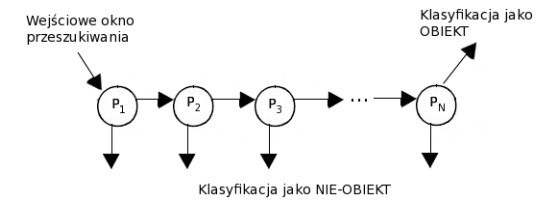
\includegraphics[width=11cm]{Obrazy/kaskadaHaar.jpg}
        \caption{Kaskada klasyfikatorów.~\cite{kaskadaHaarObraz}}
        \label{fig.kaskadaHaar}
    \end{figure}
    Okna są oznaczone jako P1, P2, \ldots, Pn.
    Gdy dane okno wykryje obiekt, przechodzi do kolejnego okna w kaskadzie.
    W przeciwnym wypadku algorytm przerywa działanie i na danym obrazie nie zostaje zidentyfikowany obiekt.
    Okna są poustawiane tak, aby każde z nich klasyfikowało obiekt z różnym prawdopodobieństwem wykrycia oraz
    prawdopodobieństwem błędu.
    Składnikami wyżej wymienionego prawdopodobieństwa jest macierz pomyłek (Rysunek~\ref{fig.ConfusionMatrix}).

    \begin{figure}
        \centering
        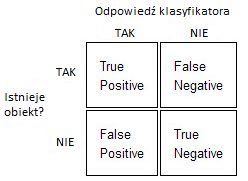
\includegraphics[width=11cm]{Obrazy/ConfusionMatrix.jpg}
        \caption{Macierz pomyłek.}
        \label{fig.ConfusionMatrix}
    \end{figure}

    Z macierzy\ref{fig.ConfusionMatrix} można odczytać czy klasyfikator poprawnie sklasyfikował dane testowe.
    W macierzy użyto 4 pojęcia:
    \begin{itemize}
        \item TP (true positive) - poprawna klasyfikacja, jako obiekt
        \item TN (true negative) - poprawna klasyfikacja, jako nie - obiekt
        \item FP (false positive) - błędna klasyfikacja jako obiekt
        \item FN (false negative) - błędna klasyfikacja jako nie - obiekt
    \end{itemize}

    Prawdopodobieństwo błędu wyliczane jest ze współczynnika FPR (false positive rate) (Wzór~\ref{wzor.fpr}).

    \large
    \begin{equation}
        FPR= \frac{FP}{FP+TN}
        \label{wzor.fpr}
    \end{equation}
    \normalsize

    Natomiast prawdopodobieństwo wykrycia obiektu wyliczane jest ze współczynnika TPR (true positive ratio)
    (Wzór~\ref{wzor.tpr})
    \large
    \begin{equation}
        TPR= \frac{TP}{TP+FN}
        \label{wzor.tpr}
    \end{equation}
    \normalsize

    Pierwsze okna posiadają klasyfikatory o słabszym TPR oraz FPR niż kolejne okna.
    Oznacza to, że prawdopodobieństwo TPR w oknie $P_{x-1}$ jest mniejsze od tego w $P_{x}$.
    Natomiast prawdopodobieństwo FPR w oknie $P_{x-1}$ jest większe od tego w $P_{x}$.
    Ostatnie okna mają największy współczynnik TPR oraz najmniejszy FRP ze wszystkich.
    Takie ustawienie okien ma na celu wstępne przepuszczenie przez okna obrazów,
    które z dużym prawdopodobieństwem zawierają szukany obiekt.
    Natomiast ostatnie okna w kaskadzie analizują niewielką część obrazu wejściowego.
    %Opis kaskady
    %    The overall form of the detection process is that of a degenerate decision tree, what we call a “cascade” (see Figure 4). A positive result from the first classifier triggers the
    %    evaluation of a second classifier which has also been adjusted to achieve very high detection rates. A positive result
    %    from the second classifier triggers a third classifier, and so
    %    on. A negative outcome at any point leads to the immediate
    %    rejection of the sub-window.
    %    Stages in the cascade are constructed by training classifiers using AdaBoost and then adjusting the threshold to
    %    minimize false negatives. Note that the default AdaBoost
    %    threshold is designed to yield a low error rate on the training data. In general a lower threshold yields higher de
    %    W ostatniej fazie stosowany jest algorytm kaskady klasyfikatorów.
    %    Klasyfikatory są podzielone na grupy i
    %    połączone ze sobą kaskadowo.
    %    W algorytmie każda grupa może podjąć dwie decyzje - przekazanie danych z klasyfikatorów
    %    do kolejnej grupy lub ich odrzucenie.
    %    Ma to na celu odrzucenie wielu negatywnych danych z klasyfikatorów~\cite{cascade}.

    Biblioteka OpenCV zawiera wytrenowane klasyfikatory, które zostały użyte w tej pracy magisterskiej.
    Wykorzystano
    je do wykrycia twarzy, ust oraz oczu.
    Klasyfikatory mają postać plików xml, które można znaleźć na oryginalnym
    repozytorium projektu OpenCv.

    %1600 wyrazow
    \section{Wyznaczanie stref}\label{sec:wyznaczanieStref}
    %Wzory na wyznaczenie stref z "okienek"
    Przed wyznaczeniem stref zmarszczkowych należy zidentyfikować na twarzy oczy oraz nos
    (Rysunek~\ref{fig.wykrywanieOczuNosa}).
    \begin{figure}
        \centering
        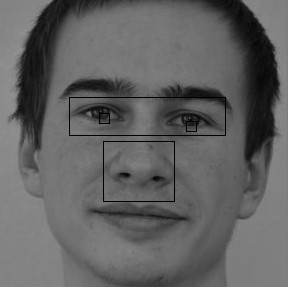
\includegraphics[width=8cm]{Obrazy/wykrywanieOczuNosa.jpg}
        \caption{Wykryty nos oraz oczy.}
        \label{fig.wykrywanieOczuNosa}
    \end{figure}


    Należy podkreślić, że algorytm przerywa działanie jeśli nie zostanie wykryta twarz, oczy lub nos.

    Gdy zostanie wykryty obszar twarzy, oczu oraz nosa wyznaczone zostaje sześć stref zmarszczkowych
    (Rysunek~\ref{fig.wykrywanieStrefZmarszczkowych}).

    \begin{figure}
        \centering
        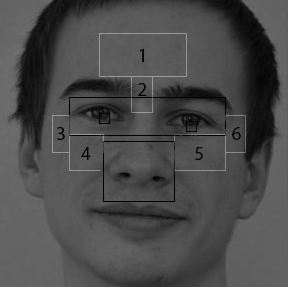
\includegraphics[width=8cm]{Obrazy/strefyZmarszczkowe.jpg}
        \caption{Strefy zmarszczkowe widoczne w białych prostokątach.}
        \label{fig.wykrywanieStrefZmarszczkowych}
    \end{figure}

    Strefy zmarszczkowe są na czole (Strefa ,,1''), w górnej części nosa (Strefa ,,2''), górnej części policzków
    (Strefa ,,4'' i ,,5'') oraz w okolicach powiek (Strefa ,,3'' i ,,6'').
    To właśnie te miejsca zostały uznane przez autorów książki ,,Age Estimation from Face Image using Wrinkle
    Features''~\cite{wrinkleFeatures} za najbardziej znaczące w detekcji wieku.

    Po detekcji oczu należy zmierzyć odległość pomiędzy środkiem lewego oka ($x_{l},y_{l}$),
    a prawego ($x_{p},y_{p}$)
    (Wzór~\ref{wzor.odlegloscPomiedzyOczami}).
    \large
    \begin{equation}
        d= \sqrt{\left ( x_{r} - x_{l} \right )^{2}+\left (y_{r} - y_{l}  \right )^{2}}
        \label{wzor.odlegloscPomiedzyOczami}
    \end{equation}
    \normalsize

    Odległość d służy do wyznaczanie strefy znajdującej się na czole (Rysunek~\ref{fig.wyznaczenieCzola}).


    \begin{figure}
        \centering
        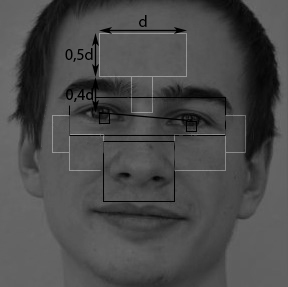
\includegraphics[width=11cm]{Obrazy/wyliczenieCzolka.jpg}
        \caption{Wyznaczenie strefy znajdującej się na czole.}
        \label{fig.wyznaczenieCzola}
    \end{figure}

    Autorzy~\cite{wrinkleFeatures} algorytmu założyli, że odległość od linii oczu do linii brwi wynosi $0,4 * d$,
    natomiast wymiary ,,strefy czoła'' wynoszą $d \times 0,5d$.

    Na Rysunku~\ref{fig.wspolrzedneDoWyliczeniaStref} przedstawione są współrzędne, które są pomocne w wyznaczaniu
    stref zmarszczkowych.

    \begin{figure}
        \centering
        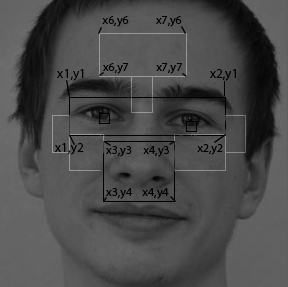
\includegraphics[width=9cm]{Obrazy/wspolrzedneDoWyliczeniaStref.jpg}
        \caption{Pomocnicze współrzędne do wyliczania stref zmarszczkowych.}
        \label{fig.wspolrzedneDoWyliczeniaStref}
    \end{figure}

    Strefa 2 została wyznaczona dzięki znajomości położenia prawego oka, dystansu między oczami oraz strefy ,,1''.
    Każda strefa może być wyznaczona przez jeden punkt (Rysunek~\ref{fig.wykrywanieStrefZmarszczkowychPunkty})
    oraz jej wymiary.

    \begin{figure}
        \centering
        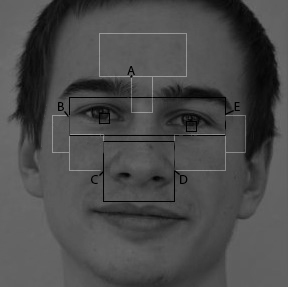
\includegraphics[width=8cm]{Obrazy/wykrywanieStrefZmarszczkowychPunkty.jpg}
        \caption{Punkty wyznaczające położenie stref.}
        \label{fig.wykrywanieStrefZmarszczkowychPunkty}
    \end{figure}

    Współrzędna x punktu A została wyznaczona ze wzoru~\ref{wzor.punktXA}

    \large
    \begin{equation}
        x_{A}=x_{6} + 0,375 \times d
        \label{wzor.punktXA}
    \end{equation}
    \normalsize
    , gdzie $x_{6}$ to współrzędna z Rysunku~\ref{fig.wspolrzedneDoWyliczeniaStref}.
    Natomiast $d$ jest odległością pomiędzy oczami (Wzór~\ref{wzor.odlegloscPomiedzyOczami}).

    Współrzędna y punktu A - Wzór~\ref{wzor.punktYA}:

    \large
    \begin{equation}
        y_{A}=y_{7}
        \label{wzor.punktYA}
    \end{equation}
    \normalsize
    Współrzędna $y_{7}$ analogicznie jak $x_{6}$ znajduje się na Rysunku~\ref{fig.wspolrzedneDoWyliczeniaStref}.

    Zakładając, że prawe oko ma współrzędne $x_{o}$ oraz  $y_{o}$ wysokość strefy 2 wyznaczana jest w poniższy sposób
    (Wzór~\ref{wzor.punktHA}).
    \large
    \begin{equation}
        h_{A}=y_{o}-y_{7}
        \label{wzor.punktHA}
    \end{equation}
    \normalsize

    Natomiast szerokość strefy 2 oblicza się następująco: (Wzór~\ref{wzor.punktWA}):
    \large
    \begin{equation}
        w_{A}=0,25 * d
        \label{wzor.punktWA}
    \end{equation}
    \normalsize
    Wartość 0,25 ze wzoru~\ref{wzor.punktWA} została dobrana empirycznie.

    Współrzędne punktu C (strefa 4) zostają wyznaczone ze Wzoru~\ref{wzor.punktXC} oraz~\ref{wzor.punktYC}.
    \large
    \begin{equation}
        x_{C}=x_{3}
        \label{wzor.punktXC}
    \end{equation}
    \normalsize

    \large
    \begin{equation}
        y_{C}= \frac{y_{4} - y_{3}}{2}
        \label{wzor.punktYC}
    \end{equation}
    \normalsize

    Wysokość oraz szerokość strefy 4 (Wzór~\ref{wzor.punktHC} oraz~\ref{wzor.punktWC})

    \large
    \begin{equation}
        h_{C}=y_{C} - y_{3}
        \label{wzor.punktHC}
    \end{equation}
    \normalsize

    \large
    \begin{equation}
        w_{C}= x_{3} - x_{1}
        \label{wzor.punktWC}
    \end{equation}
    \normalsize

    Strefa 5 zawiera punkt D - Wzór~\ref{wzor.punktXD} oraz~\ref{wzor.punktYD}.

    \large
    \begin{equation}
        x_{D}=x_{4}
        \label{wzor.punktXD}
    \end{equation}
    \normalsize

    \large
    \begin{equation}
        y_{D}= y_{C}
        \label{wzor.punktYD}
    \end{equation}
    \normalsize

    Dla strefy 5 wyznacza sie wysokość (Wzór~\ref{wzor.punktHD}) oraz szerokość na podstawie wzoru (Wzór~\ref{wzor.punktWD}).

    \large
    \begin{equation}
        h_{D}=h_{C}
        \label{wzor.punktHD}
    \end{equation}
    \normalsize

    \large
    \begin{equation}
        w_{D}= x_{2} - x_{4}
        \label{wzor.punktWD}
    \end{equation}
    \normalsize

    Strefa 3 zawiera punkt B wyznaczany ze Wzorów~\ref{wzor.punktXB} i~\ref{wzor.punktYB}

    \large
    \begin{equation}
        x_{B}=x_{1}
        \label{wzor.punktXB}
    \end{equation}
    \normalsize

    \large
    \begin{equation}
        y_{B}= \frac{y_{2} - y_{1}}{2}
        \label{wzor.punktYB}
    \end{equation}
    \normalsize

    Wysokość (Wzór~\ref{wzor.punktHB}) oraz szerokość (Wzór~\ref{wzor.punktWB}) strefy 3.

    \large
    \begin{equation}
        h_{B}=y_{C} - y_{B}
        \label{wzor.punktHB}
    \end{equation}
    \normalsize

    \large
    \begin{equation}
        w_{B}= w_{C} * 0,4
        \label{wzor.punktWB}
    \end{equation}
    \normalsize

    Na samym końcu zostaje wyznaczona strefa 6.
    Wyznaczona zostaje współrzędna E - Wzór~\ref{wzor.punktXE} i~\ref{wzor.punktYE}.
    \large
    \begin{equation}
        x_{E}=x_{2}
        \label{wzor.punktXE}
    \end{equation}
    \normalsize

    \large
    \begin{equation}
        y_{E}= y_{B}
        \label{wzor.punktYE}
    \end{equation}

    Szerokość oraz wysokość strefy 6.

    \large
    \begin{equation}
        h_{E}=h_{B}
        \label{wzor.punktHE}
    \end{equation}
    \normalsize

    \large
    \begin{equation}
        w_{E}= w_{D} * 0,4
        \label{wzor.punktWE}
    \end{equation}
    \normalsize

    Należy zauważyć, że szerokość stref 3 i 6 jest pomnożona przez 0,4 szerokości odpowiednio
    stref 4 i 5.
    Wartość ,,0,4'' została dobrana empirycznie.
    \section{Wykrywanie zmarszczek - detektor Canny}\label{sec:wykrywanie-zmarszczek---detektor-canny}
    %todo opis detektora z wiki angielskiej
    %moze troche opisu configu Cannego od Anielskiej
    Następnym krokiem algorytmu po wyznaczeniu stref zmarszczkowych jest wyodrębnienie zmarszczek.
    W celu identyfikacji zmarszczek zastosowano detektor Canny.
    Detekcja krawędzi pozwala na wyodrębnienie wielu użytecznych cech z obrazu,
    ponadto znacznie zmniejsza ilość informacji do przetworzenia przez algorytm,
    który wyodrębnia cechy z obrazu.
    Istnieje wiele detektorów krawędzi,
    jednak detektor Canny jest jednym z najbardziej dokładnych i niezawodnych.
    Metoda detekcji została opracowana przez Johna F. Canny w 1986 roku.
    Oprócz samej implementacji algorytmu jego twórca zaprezentował teorię obliczeniową,
    która wyjaśnia działanie tej metody. Ponadto Canny zauważył,
    że wymagania dotyczące implementacji detekcji krawędzi są podobne do siebie w wielu systemach wizyjnych.
    W związku z powyższym jego algorytm może zostać skutecznie zastosowany w różnych systemach wizyjnych.
    Poniżej przedstawiono najważniejsze zasady,
    które są niezbędne do dobrej detekcji krawędzi w opisywanym algorytmie:
    \begin{itemize}
        \item Detekcja krawędzi z niskim prawdopodobieństwem błędu:
        Oznacza to, że algorytm powinien wykryć jak najwięcej krawędzi, które rzeczywiście istnieją.
        Natomiast ilość krawędzi wykrytych błędnie powinna być jak najmniejsza.
        \item Precyzja detekcji: Algorytm powinien precyzyjnie zlokalizować krawędź.
        \item Brak redundantnych detekcji:
        Krawędź powinna być zlokalizowana jednokrotnie,
        a szum na obrazie nie powinien generować dodatkowych krawędzi.
    \end{itemize}
    W algorytmie detekcji Canny używa rachunku wariacyjnego.
    Rachunek wariacyjny to dziedzina analizy matematycznej, która
    analizuje przestrzenie funkcyjne i znajduje w nich ekstrema funkcjonałów.
    Funkcjonały natomiast przekształcają przestrzeń wektorową na liczby rzeczywiste.
    Zatem rachunek wariacyjny ma za zadanie pomóc w znalezieniu charakterystycznej funkcji,
    dla której funkcjonał przyjmuje wartość ekstremalną.
    Algorytm detektora jest podzielony na kilka kroków~\cite{Canny}:
    \begin{itemize}
        \item Redukcja szumów na obrazie filtrem Gaussa.
        \item Szukanie gradientów jasności.
        \item Zastosowanie techniki zmniejszania grubości krawędzi.
        \item Likwidacja krawędzi o małym gradiencie jasności.
        \item Filtracja poprzez histerezę.
    \end{itemize}
    \subsection{Redukcja szumów na obrazie filtrem Gaussa}\label{subsec:redukcja-szumów-na-obrazie-filtrem-gaussa}
    Szum na obrazie to piksele o losowym kolorze, jasności oraz umiejscowieniu (współrzędnych na obrazie).
    Takie piksele są nadmiarowymi informacjami o obrazie oraz stanowią efekt uboczny przetwarzania obrazu
    przez matrycę cyfrową (Rysunek~\ref{fig.lenkaSzumy}).

    \begin{figure}
        \centering
        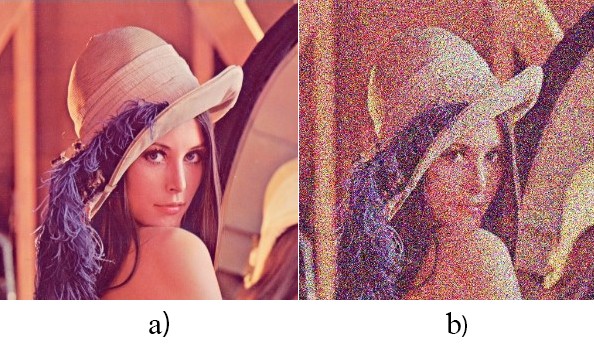
\includegraphics[width=11cm]{Obrazy/lenkaSzumy.jpg}
        \caption{a) Obraz z nieznaczną ilością szumów b) Obraz ze znaczną ilością szumów.~\cite{lenkaSzumy}}
        \label{fig.lenkaSzumy}
    \end{figure}

    Efekt szumu jest spotykany również w fotografii analogowej.
    W fotografii cyfrowej szum wzrasta na skutek zwiększania czułości matrycy lub przez wzrost jej temperatury.
    Redukcję szumów można uzyskać stosując filtr Gaussa.
    Splot filtru Gaussa z obrazem daje w wyniku wygładzony obraz ze zmniejszoną ilością szumów.
    Filtr Gaussa może mieć różne wymiary, natomiast
    Najczęściej stosowanym jest 5x5.
    Rozmiar filtra ma wpływ na wydajność wygładzania obrazu, a co za tym idzie na czułość wykrywania szumu~\cite{Canny}.
    \subsection{Szukanie gradientów jasności}\label{subsec:szukanie-gradientów-jasności}
    Istotnym parametrem w wykrywaniu krawędzi jest gradient jasności.
    Określa on jak bardzo zmienia się jasność danego piksela względem sąsiadujących pikseli.
    Gradient jasności otrzymany zostaje ze wzoru~\ref{wzor.gradientJasnosci}:
    \large
    \begin{equation}
        G = \sqrt{G_{x}^{2} + G_{y}^{2}}
        \label{wzor.gradientJasnosci}
    \end{equation}
    \normalsize
    gdzie Gx jest zmianą jasności danego piksela w kierunku poziomym, a Gy w kierunku pionowym.
    Kierunek gradientu opisuje wzór~\ref{wzor.kierunekGradientu}
    \large
    \begin{equation}
        \Theta = atan2(G_{y}, G_{x})
        \label{wzor.kierunekGradientu}
    \end{equation}
    \normalsize
    Krawędzie na obrazie charakteryzują się pewną zmianą jasności na danym obszarze obrazu.
    Krawędź na obrazie może być położona pod różnym kątem.
    Opisywany detektor używa czterech filtrów w celu wykrycia pionowych, poziomych oraz ukośnych krawędzi.

    Kierunek gradientu jest zaokrąglony do jednego z filtrów kierunku: poziomego ($\Theta = 0^{\circ}$),
    pionowego($\Theta = 90^{\circ}$) lub ukośnego ($\Theta = 45^{\circ}$
    lub $\Theta = 135^{\circ}$ stopni).
    Każdy piksel obrazu otrzymuje wartość gradientu (Wzór~\ref{wzor.gradientJasnosci})
    oraz kierunek - zgodny z powyższym filtrem kierunku.
    W wyniku tego działania zostaje otrzymany obraz gradientowy~\cite{Canny}.
    \subsection{Zastosowanie techniki zmniejszania grubości
    krawędzi}\label{subsec:zastosowanie-zmniejszania-grubości-krawędzi}
    Zmniejszanie grubości krawędzi służy do filtracji krawędzi powstałych po poprzednim kroku.
    Krawędzie wykryte za pomocą gradientu są rozmyte (nieostre).
    Dzięki technice zmniejszania grubości krawędzi można odszukać na małym obszarze gradienty o największej wartości.
    Wszystkie inne, o mniejszej wartości, są ignorowane.
    Dzięki temu pozostawia się gradienty o największej wartości, które identyfikują najostrzejsze krawędzie.
    Algorytm operuje na obrazie gradientowym powstałym jako wynik działania algorytmu opisanego w sekcji~\ref{subsec:szukanie-gradientów-jasności}
    Działa on następująco:

    Odczytana zostaje wartość gradientu oraz jego kierunek dla danego piksela.
    Następnie wartość gradientu porównuje się z wartościami gradientu dla
    dwóch sąsiednich pikseli.
    Pierwszy sąsiedni piksel jest wyznaczony przed aktualny kierunek gradientu, a drugi przez kierunek przeciwny.
    Jeśli wartość danego piksela jest największa spośród pikseli wzdłuż wyżej wymienionych linii,
    to dany piksel należy do najostrzejszej krawędzi~\cite{Canny}.

    \subsection{Filtracja krawędzi o małym gradiencie jasności}\label{subsec:filtracja-krawędzi-o-małym-gradiencie-jasności}
    Zastosowanie techniki zmniejszania grubości krawędzi pozostawia na obrazie wiele krawędzi, które są wygenerowane przez szum i zmiany
    kolorów.
    Kolejnym krokiem jest filtracja powyższych krawędzi, gdyż są one nadmiarowe.
    W tym celu ustawiany jest pewien próg, zwany progiem małym.
    Oprócz progu małego ustawiany jest również próg duży w celu wyodrębnienia krawędzi o wysokim gradiencie jasności.
    Jeśli wartość gradientu dla danej krawędzi jest mniejsza od progu małego, to zostaje ona usunięta.
    W przypadku, gdy wartość jest większa od progu małego, ale mniejsza od progu dużego, dana krawędź
    zostaje oznaczona jako słaba.
    Krawędź oznacza się jako mocną, gdy wartość gradientu dla niej jest większa od wartości progu dużego~\cite{Canny}.

    \subsection{Filtracja poprzez histerezę}\label{subsec:filtracja-poprzez-histerezę}
    W wyniku działania algorytmu do tej pory zostały uzyskane słabe oraz mocne krawędzie.
    Mocne krawędzie zostaną oznaczone jako prawdziwe krawędzie znajdujące się na obrazie.
    Słabe krawędzie mogą być częścią mocnych krawędzi, ale
    mogą również zostać wygenerowane przez szum lub zmiany kolorów.
    Krawędzie tego typu nie są prawdziwymi krawędziami w obrazie, więc w ostatnim kroku algorytmu powinny zostać
    przefiltrowane.
    Słabe krawędzie, które są powiązane z mocnymi znajdują się w najbliższym sąsiedztwie mocnych krawędzi.
    W celu odnalezienia tych powiązań pomiędzy krawędziami zostaje zastosowana analiza spójności krawędzi.
    Jeśli zostaje zidentyfikowane powiązanie pomiędzy mocną, a słabą krawędzią, to słabą krawędź pozostawia się w obrazie.
    W przypadku, gdy słaba krawędź nie jest powiązana z żadną mocną krawędzią - zostaje usunięta~\cite{Canny}.

    \section{Wyliczanie wrinkle feature}\label{sec:wyliczanieWrinkleFeature}
    W wyniku działania detektora Cannego, który został opisany w sekcji~\ref{sec:wykrywanie-zmarszczek---detektor-canny}
    wygenerowany zostaje obraz binarny z wyodrębnionymi krawędziami.
    Obraz binarny zawiera piksele o dwóch wartościach jasności pikseli.
    Piksel może być albo biały albo czarny.
    Krawędzie można rozpoznać jako białe piksele, natomiast czarne piksele oznaczają brak krawędzi (Rysunek~\ref{fig.mojaTwarzGray}).

    \begin{figure}
        \centering
        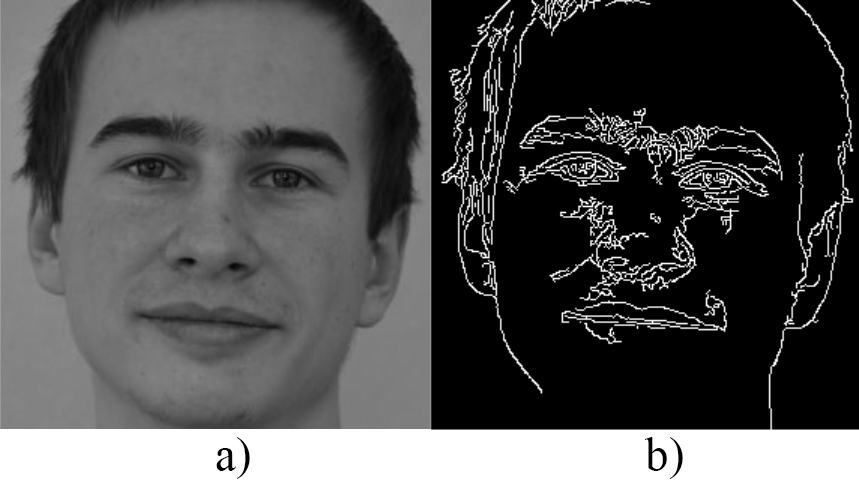
\includegraphics[width=11cm]{Obrazy/mojaTwarzGray.jpg}
        \caption{a) Oryginalny obraz b) Obraz z wykrytymi krawędziami.}
        \label{fig.mojaTwarzGray}
    \end{figure}

    Na Rysunku~\ref{fig.mojaTwarzGray} widoczne są krawędzie, które wyróżniają tło od twarzy.
    Ponadto widoczne są poszczególne części twarzy tj. nos, oczy, brwi.
    Można także zauważyć dodatkowe krawędzie w strefach zmarszczkowych (Sekcja~\ref{sec:wyznaczanieStref}),
    które identyfikują zmarszczki.
    Ilość białych pikseli w strefach zmarszczkowych jest wprost proporcjonalna do ilości zmarszczek na twarzy danej
    osoby.

    Z każdej strefy zmarszczkowej obliczany jest stosunek ilości białych pikseli do wszystkich
    pikseli (Wzór ~\ref{wzor.wspolczynnikZmarszczek}).
    \large
    \begin{equation}
        W_{s1} = \frac{PB_{s1}}{PW_{s1}}
        \label{wzor.wspolczynnikZmarszczek}
    \end{equation}
    \normalsize
    , gdzie $W_{s1}$ jest stosunkiem białych pikseli do wszystkich w strefie 1,
    $PB_{s1}$ - suma białych pikseli w strefie 1, $PW_{s1}$ - suma wszystkich pikseli w strefie 1.
    Analogicznie obliczane są stosunki pikseli dla pozostałych stref.
    Ostatnim etapem jest sumowanie wszystkich stosunków pikseli (Wzór~\ref{wzor.wrinkleFeature}).
    \large
    \begin{equation}
        WF = W_{s1} + W_{s2} + W_{s3} + W_{s4} + W_{s5} + W_{s6}
        \label{wzor.wrinkleFeature}
    \end{equation}
    \normalsize
    , gdzie WF to wrinkle feature - parametr określający ilość zmarszczek dla danej osoby.

    \section{Algorytm trenowania}\label{sec:algorytmTrenowania}
    W celu skonstruowania programu wyznaczającego wiek na podstawie tekstury należy wcześniej zbadać zależność ilości
    zmarszczek od wieku.
    W tym celu należy posiadać odpowiednią bazę zdjęć, na których można przeprowadzić wyżej wspomniane badania.

    Jest wiele darmowych źródeł obrazów twarzy.
    Najczęściej używane bazy to FG-NET oraz MORTH II, które
    zawierają dziesiątki tysięcy zdjęć.
    Zdjęcia są różnej jakości i nie każda baza zdjęć nadaje się do konkretnych badań~\cite{khryashchevGanin}.
    Przy realizacji tej pracy wykorzystana została baza UTKFace,
    ponieważ w jej przypadku ścieżka pliku każdego obrazu zawiera informacje na temat rzeczywistego wieku.
    W związku z powyższym z każdego zdjęcia z tej bazy otrzymywano dwie informacje - rzeczywisty wiek danej osoby oraz
    współczynnik zmarszczek.
    Następnie dla całej bazy wygenerowano zbiór danych, który w dalszej kolejności był odpowiednio analizowany w celu
    sprawdzenia zależności pomiędzy współczynnikiem zmarszczek, a wiekiem. Wyżej wymieniony proces nazywany jest
    także trenowaniem zbioru danych.

    Autorzy algorytmu w celu analizy wyżej wygenerowanego zbioru danych wykorzystali algorytm grupowania -
    Fuzzy C-Means.
    W wyniku działania tego algorytmu otrzymuje się dane, dzięki którym na podstawie współczynnika zmarszczek można
    oszacować wiek~\cite{wrinkleFeatures}.
    \section{Grupowanie danych - Fuzzy C-Means oraz wyznaczanie wieku}\label{sec:grupowanieDanych}
    %    https://pl.wikipedia.org/wiki/Analiza_skupień
    %    https://en.wikipedia.org/wiki/Cluster_analysis
    %    https://sci-hub.tw/10.1109/ICCSA.2019.000-1
    %    https://www.researchgate.net/publication/329424581_Data_clustering
    %    Podac rozne przyklady algorytmow - hierarchiczne, niehierarchiczne
    %todo mozna dopisac o roznych odleglosciach stosowanych do przydzielania do klastrow
    Grupowanie danych, zwane również klasteryzacją, jest szeroko stosowane w uczeniu maszynowym, rozpoznawaniu wzorców,
    analizie obrazu, bioinformatyce, kompresji danych czy w grafice komputerowej.
    Polega na podzieleniu dużego zbioru danych na grupy.
    Powyższe grupy zawierają dane, które są podobne do siebie~\cite{clusterWstep}.

    Klasteryzacja nie jest algorytmem, lecz zadaniem, które może zostać wykonane na wiele sposobów.
    Jest również iteracyjnym procesem odkrywania danych w celu odnalezieniu relacji pomiędzy nimi.

    Odpowiedni algorytm grupowania i ustawienia parametrów (w tym parametrów
    takie jak funkcja odległości lub liczba oczekiwanych grup)
    zależą od zestawu danych i sposobu wykorzystania wyników.
    Dane nieraz muszą zostać przefiltrowane lub potrzebna jest zmiana parametrów grupowania w celu osiągnięcia
    zamierzonego efektu~\cite{clusterWstep}.

    Algorytmy różnią się pod względem implementacji grupowania czy wydajności.
    Najczęściej grupa jest definiowana przez jak najmniejszą odległość pomiędzy jej członkami.
    Zarazem odległość pomiędzy członkami grupy jest głównym parametrem klasteryzacji hierarchicznej.
    Istnieje również wiele innych modeli grupowania.
    Jednym z nich jest model centroidowy,
    który zakłada, że każda grupa jest zdefiniowana przez jeden wektor, posiadający wartość średnią.
    Istnieją też modele, które opierają się na sieciach neuronowych.
    Ich podstawą jest założenie, że dane grupują się za pomocą nienadzorowanych sieci neuronowych.
    Spotykany jest także model oparty o rozkłady statystyczne.

    Klasteryzacja może być twarda lub miękka.
    Twarda klasteryzacja oznacza, że każdy element danych może należeć tylko do jednej grupy.
    Natomiast w przypadku miękkiej klasteryzacji każdy element danych może w pewnym stopniu należeć do każdej z grup.
    Autorzy algorytmu szacowania wieku opisywanego w niniejszej pracy zastosowali grupowanie metodą Fuzzy C-means.
    Należy ona do grupy modeli centroidowych~\cite{clusterWstep}. W Fuzzy C-means zastosowano klasteryzacje miękką.

    %todo - dokladny opis jak to dziala
    %    https://sci-hub.tw/10.1007/s12046-019-1166-1
    %pozniej opisac co otrzymalismy w wyniku dzialania algorytmu, ze tam byly centroidy wraz z wartoscia
    Algorytm Fuzzy C-means został stworzony w 1973 przez J. C. Dunn. Została opisana ona w książce
    ,,A Fuzzy Relative of the ISODATA Process and Its Use in Detecting Compact Well-Separated Clusters''.

    Klasteryzacja Fuzzy C-means dzieli zbiór X (Wzór~\ref{wzor.zbiorX}):
    \large
    \begin{equation}
        X:=\{x_{1},x_{2},x_{3},\ldots,x_{n}\}\subset \mathbb{R}
        \label{wzor.zbiorX}
    \end{equation}
    \normalsize
    W parametrze algorytmu zostaje ustalona liczba grup c.
    Każda grupa posiada charakterystyczną wartość nazywana centroidem $p_{j}\subset \mathbb{R}$.
    Jak zostało wspomniane na początku tego rozdziału, w algorytmie C-means zastosowana jest miękka klasteryzacja.
    Każdy element danych ma przypisywany wektor $U_{i}$ przynależności do grupy (Wzór~\ref{wzor.wektorPrzynaleznosci}).
    \large
    \begin{equation}
        U_{i}=(u_{i1}, u_{i2}, u_{i3}, \ldots, u_{ic})
        \label{wzor.wektorPrzynaleznosci}
    \end{equation}
    \normalsize
    , gdzie $u_{i1}$ oznacza stopień przynależności elementu $x_{i}$ do grupy 1.
    Analogicznie $u_{i2}$ oznacza stopień przynależności elementu $x_{i}$ do grupy 2.

    W pierwszym kroku zbiór centroidów P jest inicjalizowany losowo (Wzór~\ref{wzor.zbiorCentroidow}).
    \large
    \begin{equation}
        P^{0}=(p_{1}^{0}, p_{2}^{0}, p_{3}^{0}, \ldots, p_{c}^{0})
        \label{wzor.zbiorCentroidow}
    \end{equation}
    \normalsize
    W k-tym kroku algorytmu wyliczona jest macierz funkcji przynależności $U^{k} = {u_{ij}^{k}}$ (Wzór~\ref{wzor.funkcjaPrzynaleznosci}).
    \large
    \begin{equation}
        u_{ij}^{k} = \frac{1}{\sum_{k=1}^{c}\left ( \frac{\left \| x_{i} - p_{j}^{k} \right \|}{\left \|x_{i} - p_{k}^{k}  \right \|} \right )^{\frac{2}{m-1}}}
        \label{wzor.funkcjaPrzynaleznosci}
    \end{equation}
    \normalsize
    Wyrażenie $\left \| x_{i} - p_{j} \right \|$ oznacza odległość Euklidesową pomiędzy elementem $x_{i}$ a
    centroidem $p_{j}$. Parametr ,,m'' jest nazywany współczynnikiem rozmycia. Współczynnik ten może być w zakresie
    od 1 do nieskończoności, jednak w większości przypadków jest równy 2.

    W kroku $(k+1)^{th}$ centroid $p_{j}^{(k+1)}$ jest uaktualniany według Wzoru~\ref{wzor.kaPLusJeden}.
    \large
    \begin{equation}
        p_{j}^{(k+1)}=\frac{\sum_{i=1}^{n}u_{ij}^{(k+1)m}x_{j}}{\sum_{i=1}^{n}u_{ij}^{(k+1)m}}
        \label{wzor.kaPLusJeden}
    \end{equation}
    \normalsize
    Algorytm w kolejnych iteracjach minimalizuje kryterium $J(U,P)$ podane Wzorem~\ref{wzor.kryteriumFCM}:

    \large
    \begin{equation}
        J(U,P)= \sum_{i=1}^{n}\sum_{j=1}^{c}u_{ij}^{m}\left \| x_{i}-p_{j} \right \|^{2}
        \label{wzor.kryteriumFCM}
    \end{equation}
    \normalsize
    Iteracje kończą się, gdy zostanie osiągnięty warunek opisany Wzorem~\ref{wzor.koniecIteracjiWarunek}
    \large
    \begin{equation}
        \left \| J^{(k+1)}(U,P) - J^{(k)}(U,P)) \right \| < \epsilon
        \label{wzor.koniecIteracjiWarunek}
    \end{equation}
    \normalsize
    , gdzie $\epsilon > 0$. Parametr $\epsilon$ jest parametrem ustawianym przed uruchomieniem klasteryzacji.
    W niektórych implementacjach istnieje możliwość zakończenia działania algorytmu po określonej liczbę iteracji,
    jeśli wcześniej nie zostanie osiągnięte kryterium ze Wzoru~\ref{wzor.koniecIteracjiWarunek}.

    Po zakończeniu działania wyżej opisanego algorytmu zostaje wyliczony wektor przynależności $U$
    (Wzór~\ref{wzor.wektorPrzynaleznosci}).
    %    U_{i}=(u_{i1}, u_{i2}, u_{i3}, \ldots, u_{ic})
    Zakładając, że suma wektora przynależności $U_{i}$, dla elementu $x_{i}$ jest opisana
    Wzorem~\ref{wzor.sumaWektorPrzynaleznosci}
    \large
    \begin{equation}
        \sum_{j=0}^{j=c} u_{ij}=1
        \label{wzor.sumaWektorPrzynaleznosci}
    \end{equation}
    \normalsize
    , gdzie c oznacza liczbę klastrów.
    Element $x_{i}$ będzie należał do klastru k, jeśli $u_{ik}$ ma największą wartość w wektorze $U_{i}$.

    W tym akapicie zostanie przedstawiony algorytm trenowania za pomocą Fuzzy C-means.
    Z każdego zdjęcia ,,i'' otrzymywane są dane dotyczące rzeczywistego wieku $A_{i}$ oraz parametr wrinkle feature
    $F_{i}$.
    W algorytmie Fuzzy C-means są grupowane dane zawierające wartości wrinkle feature $F_{i}$.
    Jak wiadomo z powyższego opisu algorytmu Fuzzy C-means, każdy element (w tym przypadku $F_{i}$) ma określony stopień
    przynależności do każdego klastra. Dany element $F_{i}$ będzie należał do klastra o największym stopniu
    przynależności. Każde zdjęcie jest grupowane według wyżej opisanego algorytmu.

    Każdy klaster ma określony centroid j, który posiada parametr $P_{fj}$  oraz dodatkowy parametr - średnią
    wartość wieku $P_{aj}$. $P_{fj}$ oznacza wartość wrinkle feature dla danego centroida.
    $P_{aj}$ jest wyznaczany ze Wzoru~\ref{wzor.avgJ}.
    \large
    \begin{equation}
        P_{aj}=\frac{\sum_{}^{}A_{c}}{N_{j}}
        \label{wzor.avgJ}
    \end{equation}
    \normalsize
    , gdzie $A_{c}$ to rzeczywisty wiek osoby z obrazu c, który należy do klastru j.
    Natomiast $N_{j}$ to liczba zdjęć zaklasyfikowanych do klastru j.

    W powyższym akapicie został opisany algorytm trenowania, który generuje n centroidów, które reprezentują każdą
    grupę. Natomiast osobnym etapem jest szacowanie wieku. Należy podkreślić, że zdjęcia do testowania algorytmu szacowania wieku
    pochodzą z innej bazy obrazów niż obrazy wykorzystane w treningu. Ma to na celu eliminację błędów w testowaniu algorytmu.
    %    Każdy centroid posiada parametr
    %    W wyniku działania algorytmu wygenerowanych zostaje n grup. Każda grupa posiada centroid wraz ze średnim wiekiem.
    W pierwszej fazie działanie algorytmu jest dokładnie takie same jak w sekcjach od~\ref{sec:metodaWykrywaniaTwarzy}
    do~\ref{sec:wyliczanieWrinkleFeature}:
    Algorytm szacowania wieku w pierwszej kolejności dokonuje detekcji twarzy, oczu, ust na danym obrazie $O_{i}$.
    Jeśli powyższe elementy zostały zidentyfikowane, wyznaczane są strefy zmarszczkowe,
    a następnie zostaje wyliczony parametr wrinkle feature $F_{i}$.

    Dla parametru $F_{i}$ zostaje wyznaczony wektor przynależności do grupy
    według Wzoru~\ref{wzor.wektorPrzynaleznosci}.
    Przy założeniu dla wektoru przynależności zgodnym ze Wzorem~\ref{wzor.sumaWektorPrzynaleznosci} szacowany wiek
    $PA$
    wynosi
    (Wzór~\ref{wzor.szacowanyWiek}).
    \large
    \begin{equation}
        PA=\sum_{j=1}^{c}(u_{ij}*P_{aj})
        \label{wzor.szacowanyWiek}
    \end{equation}
    \normalsize
    , gdzie $u_{ij}$ oznacza przynależność i-tego zdjęcia do j-tego klastra, $c$ oznacza liczbę klastrów.
    Natomiast $P_{aj}$ jest średnim wiekiem dla j-tego centroida.
    %    Zbiór zdjęć użytych do treningu wynosi około 22000.
    % opisac wraz z przykladem moze jakis rysuneczek.

    %Tutaj powinno byc 5000 slow
    \chapter{Modyfikacje metody bazowej}\label{ch:modyfikacje-metody-bazowej}
    W pracy została odtworzona oryginalna praca autorów, która
    będzie dalej nazywana metodą bazową.
    W celu poprawienia wyników metody bazowej wprowadzono kilka modyfikacji, a
    w kolejnym kroku wyniki zostały porównane z pozostałymi metodami.

    Parametrem określającym jakość metody bazowej oraz metod zmodyfikowanych jest średni błąd bezwzględny,
    który został określony we Wzorze~\ref{wzor.mae}.
    \large
    \begin{equation}
        MAE = \frac{\sum_{i=1}^{n}\left | R_{i}-P_{i} \right |}{n}
        \label{wzor.mae}
    \end{equation}
    \normalsize
    , gdzie $R_{i}$ oznacza wartość rzeczywistą wieku dla i-tego zdjęcia, $n$ oznacza liczbę zdjęć testowych.
    Natomiast $P_{i}$ oznacza wartość szacowaną wieku.

    \section{Odjęcie wybranej strefy}\label{sec:odjęcie-wybranej-strefy}
    Pierwsza modyfikacja polegała na odjęciu jednej wybranej strefy. Detektor Canny oprócz zmarszczek
    wykrywa także włosy. Podczas przeglądania wielu zdjęć zauważono, że w obrębie
    strefy zmarszczek nr 2 (Obraz~\ref{fig.wykrywanieStrefZmarszczkowych}) wykrywane są części brwi oprócz samych
    zmarszczek. Generuje to błąd, dlatego wyżej wymienionej strefy nie uwzględniono w obliczeniach.
    W Sekcji~\ref{subsec:zmiana-algorytmu-względem-metody-bazowej} porównano różnice w algorytmie przed opisaną wyżej
    modyfikacją i po niej.

    \subsection{Zmiana algorytmu względem metody bazowej}\label{subsec:zmiana-algorytmu-względem-metody-bazowej}
    Przed modyfikacją metody bazowej parametr wrinkle feature był obliczany według Wzoru~\ref{wzor.wrinkleFeature},
    który jest umieszczony w Sekcji~\ref{sec:wyliczanieWrinkleFeature}.

    Po modyfikacji parametr wrinkle feature oblicza się według Wzoru~\ref{wzor.wrinkleFeature2}.
    \large
    \begin{equation}
        WF = W_{s1} + W_{s3} + W_{s4} + W_{s5} + W_{s6}
        \label{wzor.wrinkleFeature2}
    \end{equation}
    \normalsize
    Kolejną modyfikacją było zastosowanie metody HOG - Histograms of Oriented Gradients, która została opisana w Sekcji~\ref{sec:zastosowanie-metody-hog}.

    \section{Zastosowanie metody HOG}\label{sec:zastosowanie-metody-hog}
    %https://sci-hub.tw/10.2139/ssrn.3268935
    %https://www.learnopencv.com/histogram-of-oriented-gradients/
    %    https://en.wikipedia.org/wiki/Histogram_of_oriented_gradients
    %    https://hal.inria.fr/inria-00548512/document
    Metoda HOG (Histogram of Oriented Gradients) jest deskryptorem cech z obrazu.
    Deskryptor cech wyodrębnia z obrazu pewne cechy, do których należą między innymi kształty, kolory czy tekstury.
    W metodzie bazowej rolę deskryptora tego rodzaju spełnia detektor
    krawędzi Canny (Sekcja~\ref{sec:wykrywanie-zmarszczek---detektor-canny}), który wykrywa krawędzie,
    identyfikowane jako zmarszczki.
    Z kolei Histogram of Oriented Gradients jest techniką, która liczy wystąpienia kierunków gradientów jasności.
    Liczenie jest dokonywane tylko w pewnych obszarach obrazów.
    Metoda HOG została wymyślona i opisana w 1982 przez Roberta K. McConella.
    Robert K. McConell pracował w ówczesnych czasach dla firmy Wayland Research Inc.,
    a opis jego metody został zawarty w patencie ,,Method of and apparatus for pattern recognition''~\cite{patentHOG}.
    Jednak jego metoda została po raz pierwszy zaimplementowana dopiero w 2005 roku przez Navneeta Dalala i Billa Triggsa~\cite{hogZabojady}
    z francuskiego instytutu zajmującego się badaniami w zakresie informatyki i automatyki
    (INRIA - Institut national de recherche en informatique et en automatique).
    Metoda McConella została wtedy zastosowana do detekcji pieszych na zdjęciach.
    Później metoda została rozszerzona o wykrywanie ludzi w filmach wideo,
    ponadto później stosowano ją także do wykrywania zwierząt oraz pojazdów na zdjęciach.

    Metoda Histogram of Oriented Gradients opiera się na założeniu, że wygląd i kształt obiektów na obrazie może zostać
    opisany przez gradient jasności oraz jego kierunek. Jest to dobrze widoczne na
    Rysunku~\ref{fig.gradientJasnosciNaGlowie}

    \begin{figure}
        \centering
        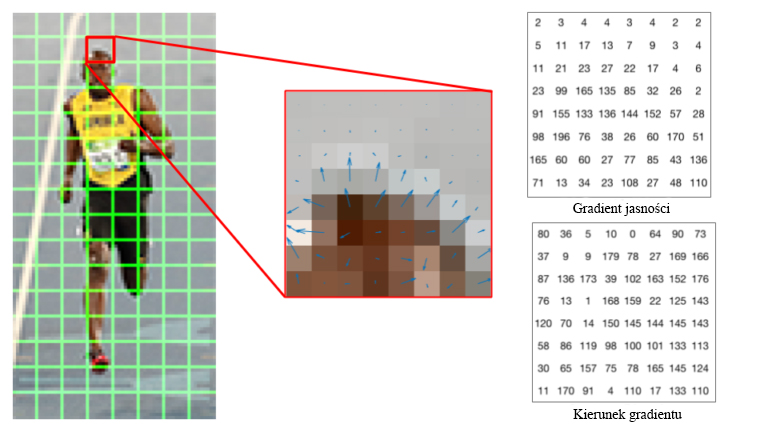
\includegraphics[width=11cm]{Obrazy/gradientJasnosciNaGlowie.jpg}
        \caption{Gradient jasności identyfikujący granicę pomiędzy głową a tłem.~\cite{hogOpenCv}}
        \label{fig.gradientJasnosciNaGlowie}
    \end{figure}
    Na granicy pomiędzy tłem, a głową sportowca widoczne są duże wartości gradientu jasności.
    W ten sposób zostaje zidentyfikowana krawędź głowy.

    Działanie algorytmu można pokrótce opisać w następujący sposób. Obraz jest dzielony na małe obszary zwane komórkami, które zwykle mają wymiar kilka na kilka pikseli.
    Dla każdego piksela w komórce tworzony jest histogram kierunków gradientu.
    Następnie histogramy są łączone w jeden wspólny deskryptor.
    Dla zwiększenia dokładności lokalne histogramy normalizowane są pod względem kontrastu.
    Realizowane jest to przez pomiar jasności obszaru zwanego blokiem, który
    składa się z kilku komórek. Normalizacja zapewnia zmniejszenia niepożądanego efektu generowanego przez
    różnice w oświetleniu różnych obszarów zdjęcia. Wspomniana sytuacja występuje na przykład, gdy zdjęcie wykonywane
    jest w nieprawidłowych warunkach oświetleniowych (Rysunek~\ref{fig.oswietlenieTwarzy}).

    W poniższym akapicie zostanie przedstawiony dokładny opis metody Histogram of Oriented Gradients.
    W pierwszej fazie obraz powinien zostać przeskalowany, tak aby jego wymiary były podzielne przez rozmiar
    pojedynczej komórki.
    (Rysunek~\ref{fig.komorkiHoga}).

    \begin{figure}
        \centering
        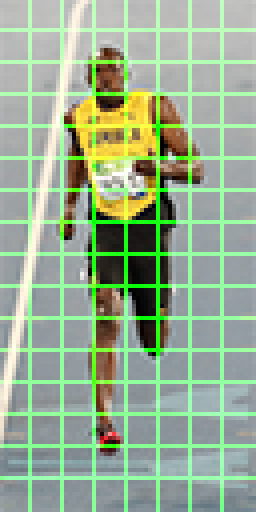
\includegraphics[width=4cm]{Obrazy/komorkiHoga.jpg}
        \caption{Komórki o rozmiarze 8x8 pikseli na zdjęciu.~\cite{hogOpenCv}}
        \label{fig.komorkiHoga}
    \end{figure}
    Warto wspomnieć, że w wielu metodach generujących deskryptory pierwszą fazą jest korekcja luminacji.
    Jednak ten krok może zostać pominięty, gdyż w późniejszym kroku stosowana jest normalizacja,
    która dokonuje korekcji luminacji cieni oraz świateł.
    W kolejnej fazie muszą zostać wyznaczone gradienty jasności.
    Wyznaczenie gradientów jasności zostało szczegółowo opisane w Sekcji~\ref{subsec:szukanie-gradientów-jasności}.
    W kolejnej fazie zostają wyznaczone histogramy gradientów dla każdej komórki.
    Na Rysunku~\ref{fig.gradientJasnosciNaGlowie} został przedstawiony wynik działania tego kroku.
    Zostają wygenerowane dwie macierze. Pierwsza zawiera informację o gradiencie jasności każdego piksela komórki,
    natomiast druga - informację o kierunku każdego gradientu.
    Wartości kierunku gradientu wyrażone są w stopniach. W metodzie Histogram of Oriented Gradients
    zastosowano kierunki gradientu bez znaku. Oznacza to, że zakres kierunków mieści się w granicach od $0^{\circ}$ do $180^{\circ}$.
    Kierunek gradientu ze znakiem posiadałby zakres od $0^{\circ}$ do $180^{\circ}$ oraz jego ujemny odpowiednik
    (od $-179^{\circ}$ do $-1^{\circ}$). Użycie kierunku gradientu bez znaku jest uzasadnione tym,
    że wartość kierunku o takiej samej wartości, lecz różnych znakach reprezentuje gradient o tym samym kierunku, lecz
    różnych zwrotach. Dla detekcji kształtów krawędzi czy kształtów istotny jest kierunek, a nie zwrot.
    Na podstawie kierunku gradientu oraz wartości gradientu jasności zostaje wygenerowany histogram gradientów.
    W parametrze wejściowym algorytmu HOG ustawiana jest ilość komórek histogramu.
    Najczęściej stosuje się 9 komórek. Każda komórka histogramu odpowiada pewnemu zakresowi kąta kierunku gradientu.
    Przykładowo dla histogramu o szerokości 9 komórek każda komórka odpowiada następującym kątom:
    $0^{\circ}$, $20^{\circ}$, $40^{\circ}$, \ldots, $160^{\circ}$ .
    Na Rysunku~\ref{fig.hogTworzenieHistogramu} przedstawiono sposób przypisywania wartości do komórek histogramu.
    \begin{figure}
        \centering
        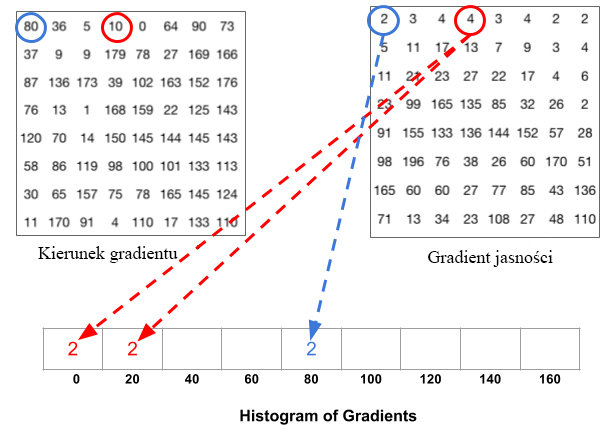
\includegraphics[width=11cm]{Obrazy/hogTworzenieHistogramu.jpg}
        \caption{Komórki o rozmiarze 8x8 pikseli na zdjęciu.~\cite{hogOpenCv}}
        \label{fig.hogTworzenieHistogramu}
    \end{figure}
    Piksel zaznaczony na niebiesko posiada gradient o wartości 2 oraz kierunek o kącie $80^{\circ}$
    Wartość gradientu zostaje dodana do komórki histogramu reprezentującego kąt $80^{\circ}$.
    Piksel zaznaczony na czerwono posiada gradient o wartości 4 oraz kierunek o kącie $10^{\circ}$.
    Wartość gradientu równa 4 zostaje rozdzielona na dwie proporcjonalne wartości: 2 oraz 2, które są dodawane do
    komórek reprezentujących kąt $0^{\circ}$ oraz $20^{\circ}$.
    Proporcje zależą od kąta gradientu i od kątów w komórkach histogramu.
    Tak jak w powyższym przypadku, jeśli wartość kąta wynosi $10^{\circ}$, wartości gradientu są przydzielane do
    komórek reprezentujące dwa kąty (w tym przypadku przedziały reprezentujące kąt od $0^{\circ}$ do
    $20^{\circ}$). W związku z tym, że powyższy kąt wynosi $10^{\circ}$, wartości dla komórek histogramu są obliczane
    według Wzoru~\ref{wzor.komorkaHistogramu1} oraz Wzoru~\ref{wzor.komorkaHistogramu2}:

    \large
    \begin{equation}
        X_{a} = \frac{A_{x}-A_{a}}{A_{b}-A_{a}}*G_{x}
        \label{wzor.komorkaHistogramu1}
    \end{equation}
    \normalsize
    , gdzie $X_{a}$ oznacza wartość przydzielaną do komórki reprezentującej mniejszy kąt (tak jak $0^{\circ}$
    dla powyższego przykładu), $A_{x}$ oznacza wartość kąta gradientu dla danego piksela (tak jak $10^{\circ}$
    dla powyższego przykładu), $A_{a}$ oznacza kąt dla komórki reprezentującej mniejszy kąt (tak jak $0^{\circ}$
    dla powyższego przykładu), $A_{b}$ oznacza kąt dla komórki reprezentującej większy kąt (tak jak $20^{\circ}$
    dla powyższego przykładu), $G_{x}$ oznacza wartość gradientu dla danego piksela (tak jak 4 dla powyższego
    przykładu).
    \large
    \begin{equation}
        X_{b} = \frac{A_{b}-A_{x}}{A_{b}-A_{a}}*G_{x}
        \label{wzor.komorkaHistogramu2}
    \end{equation}
    \normalsize
    , gdzie $X_{b}$ oznacza wartość przydzieloną dla kąta o większej wartości (tak jak $20^{\circ}$
    dla powyższego przykładu). Reszta zmiennych odpowiada zmiennym we Wzorze~\ref{wzor.komorkaHistogramu1}.
    W przypadku, gdy kąt kierunku gradientu jest większy od $160^{\circ}$ to wartość danego gradientu jest
    przydzielana proporcjonalnie do komórki $160^{\circ}$ oraz $0^{\circ}$ zgodnie ze
    Wzorem~\ref{wzor.komorkaHistogramu2}. Jednak wartość komórki $0^{\circ}$ zostaje zastąpiona kątem $180^{\circ}$,
    a wyliczona wartość zostaje przydzielona do komórki reprezentującej kąt $0^{\circ}$.
    Powyższa procedura jest powtarzana, a kolejne wartości gradientów są dodawane do aktualnych wartości przechowywanych
    w komórkach histogramu. Końcowy efekt tej fazy dostarcza histogram reprezentujący komórkę. Wartości histogramu
    dla danej komórki reprezentują część wektoru deskryptora. Deskryptor składa się z n histogramów, gdzie n oznacza
    liczbę komórek w danym obrazie.

    Kolejnym krokiem jest normalizacja bloków. Blok składa się z komórek i zazwyczaj ma wymiary 2x2 komórki.
    Gradienty jasności są czułe na zmiany oświetlenia na obrazie. Celem tej fazy algorytmu jest normalizacja oświetlania,
    aby uodpornić deskryptor na zmiany oświetlania.
    Istnieje wiele sposobów normalizacji. Zostanie tutaj opisana normalizacja za pomocą parametru L2-norm.
    Najpierw zostaje wyliczona wartość L2-norm. L2 jest wartością normalizującą wektor $v$, który reprezentuje wartości
    deskryptora dla danego bloku. Wspomniany wektor składa się z wartości zawartych w komórkach histogramu. Jak wiadomo z
    przedstawionego wyżej opisu, każdy histogram opisuje jedną komórkę, a blok zawiera n komórek.
    Przyjmując, że histogram reprezentujący komórkę posiada 9 wartości oraz rozmiar bloku
    wynosi 2x2 komórki, można wyznaczyć długość wektora $v$.
    Blok ma 2x2 komórki, więc zawiera w sobie 4 komórki. Każda komórka ma 9 wartości histogramu, więc wektor $v$ będzie
    miał długość $9x4$, czyli 36.
    L2-norm dla wektora $v$ jest obliczane według Wzoru~\ref{wzor.l2norm}
    \large
    \begin{equation}
        \left \|v  \right \|_{2}=\sqrt{\sum_{i=0}^{n}v(i)^{2}}
        \label{wzor.l2norm}
    \end{equation}
    \normalsize
    , gdzie $\left \|v  \right \|_{2}$ jest wartością L2-norm, natomiast $v(i)$ jest i-tym elementem wektora $v$.
    Normalizacja jest realizowana przy zastosowaniu Wzoru
    \large
    \begin{equation}
        v = \frac{v}{\left \|v  \right \|_{2}}
        \label{wzor.l2norm2}
    \end{equation}
    \normalsize
    , gdzie $\left \|v  \right \|_{2}$ jest wartością L2-norm dla wektora $v$. Działanie zgodne ze
    Wzorem~\ref{wzor.l2norm2} oznacza, że każdy element wektora $v$ jest dzielony przez wartość
    $\left \|v  \right\|_{2}$.
    Powyższy proces powtarza się dla wszystkich bloków.
    W wyniku działania algorytmu Histograms of Oriented Gradients wygenerowany zostaje deskryptor, czyli wektor
    reprezentujący wartości histogramów wszystkich komórek w obrazie.

    Deskryptor HOG posiada kluczową zaletę w stosunku do innych metod ekstrakcji cech.
    Jest nią odporność metody Histogram of Oriented Gradients na działanie przekształceń geometrycznych
    dzięki temu, że dokonuje działań na komórkach lokalnych.
    Przekształcenia geometryczne to działania, które przekształcają figury z jednej przestrzeni geometrycznej w drugą.
    Przykładem przestrzeni geometrycznej jest przestrzeń euklidesowa czy przestrzeń rzutowa.
    Ponadto działania na komórkach lokalnych pozwalają zmniejszyć efekt powstający przy ruchu pieszego.
    Z uwagi na powyższe zalety ta metoda nadaje się do detekcji ludzi na obrazach.

    W niniejszej pracy opisywana metoda posłużyła do wykrywania krawędzi, które informują o zmarszczkach. Dokładny sposób jej
    zaimplementowania w pracy opisuje Sekcja~\ref{subsec:zastosowanie-w-projekcie2}

    \subsection{HOG - Zastosowanie w projekcie}\label{subsec:zastosowanie-w-projekcie2}
    W poprzedniej Sekcji~\ref{sec:zastosowanie-metody-hog} został dokładnie opisany algorytm HOG, w wyniku którego
    generowany jest deskryptor dla danego obrazu.

    Omówiony wyżej deskryptor posłużył do wykrycia ilości zmarszczek w strefach zmarszczkowych. Jak wiadomo z opisu w
    Sekcji~\ref{sec:zastosowanie-metody-hog} metoda HOG pozwala na wykrywanie krawędzi w danym obrazie. Jeśli w danym
    obszarze jest dużo krawędzi, to w wektorze deskryptora będzie pewna ilość elementów tego wektora o znacznej wartości.
    Wyżej opisywane, charakterystyczne elementy wektora będą identyfikowały krawędzie w obrazie. Jak wiadomo z
    Sekcji~\ref{sec:wyliczanieWrinkleFeature} krawędzie mogą zostać zinterpretowane jako zmarszczki.
    W związku z powyższym zmodyfikowano sposób obliczenia wrinkle feature dla obrazu twarzy opierając się o
    deskryptor wygenerowany przez algorytm HOG.

    W bibliotece OpenCv zaimplementowany jest algorytm HOG, który na podstawie całego
    obrazu lub jego pewnego obszaru generuje wektor reprezentujący deskryptor. Biblioteka umożliwia ustawienie różnych parametrów HOG-a.
    Do tych parametrów zalicza się:
    \begin{itemize}
        \item rozmiar komórki w pikselach
        \item rozmiar bloku w pikselach
        \item liczba komórek w histogramie
        \item rozmiar okna - wielkość analizowanego obrazu w pikselach
    \end{itemize}

    W celu oszacowania ilości zmarszczek dla danego zdjęcia posłużono się następującym algorytmem.

    W pierwszej fazie zostały wyznaczone strefy zmarszczkowe nr 1,3,4,5,6.
    (Rysunek~\ref{fig.wykrywanieStrefZmarszczkowych}).
    Następnie dla każdej wyżej wymienionej strefy został wyznaczony deskryptor. Dla strefy 1 deskryptor jest opisany
    zmienną $v_{1}$, dla strefy 3 zmienną $v_{3}$ i tak dalej.
    Wrinkle feature jest obliczany ze Wzoru~\ref{wzor.hogWrinkleFeature}:
    \large
    \begin{equation}
        WF_{HOG} = \left \|v_{1}  \right \|_{1}+\left \|v_{3}  \right \|_{1}+\left \|v_{4}  \right \|_{1}+\left
        \|v_{5}  \right \|_{1}+\left \|v_{6}  \right \|_{1}
        \label{wzor.hogWrinkleFeature}
    \end{equation}
    \normalsize
    , gdzie $\left \|v_{1}  \right \|_{1}$ jest parametrem L1-norm dla wektora $v_{1}$. Analogicznie $\left \|v_{3}
    \right \|_{1}$  jest parametrem L1-norm dla wektora $v_{3}$.

    Parametr L1-norm dla danego wektora $v$ jest wyznaczany ze Wzoru~\ref{wzor.l1norm}:
    \large
    \begin{equation}
        \left \|v  \right \|_{1} = \sum_{i=1}^{n}\left |v(i)  \right |
        \label{wzor.l1norm}
    \end{equation}
    \normalsize
    , gdzie $v(i)$ jest i-tym elementem wektora.

    Dla każdego zdjęcia ze zbioru podobnie jak w metodzie bazowej~\ref{sec:wykrywanie-zmarszczek---detektor-canny}
    wyznaczana jest para danych $WF_{HOG}$ (Wzór~\ref{wzor.hogWrinkleFeature}) oraz wiek. Następnie wygenerowany
    zbiór danych jest trenowany za pomocą Fuzzy C-means (Sekcja~\ref{sec:grupowanieDanych}) - tak samo jak w metodzie
    bazowej.
    Wiek szacowany jest dokładnie tak samo jak w metodzie bazowej.
    Kolejna modyfikacja metody bazowej została opisana w Sekcji~\ref{sec:metoda-hog-oraz-grupowanie-knn}
    \section{Metoda HOG oraz grupowanie KNN}\label{sec:metoda-hog-oraz-grupowanie-knn}
    \subsection{Zastosowanie w projekcie}\label{subsec:zastosowanie-w-projekcie}
    %http://zsi.tech.us.edu.pl/~nowak/si/w4.pdf
    %http://www.mblachnik.pl/lib/exe/fetch.php/dydaktyka/zajecia/ai/lab/matlab/algorytm_knn.pdf
    %Trening generuje pare wiek -> wektor sumy hogow z kazdej strefy
    %Szacowanie wieku polega na generacji z testowego zdjeic pary jw. i za pomoca KNN przydzielenie do jakiejs klasy
    %    - czytaj wieku.
    %zdefiniowac problem odleglosci oraz jak bedzie ta odleglosc liczona dla wektorow (Euclidan) : http://mathonline.wikidot.com/the-distance-between-two-vectors
    %jak wyglada trenowanie danych, przeprowadzenie normalizacji itp (ze jest opcjonalne) wzory itp:
    %http://www.mblachnik.pl/lib/exe/fetch.php/dydaktyka/zajecia/ai/lab/matlab/algorytm_knn.pdf
    % wybor parametru - k jak wplywa
    Kolejna modyfikacja polegała na zmianie sposoby wyznaczania wrinkle feature.
    W Sekcji \ref{subsec:zastosowanie-w-projekcie2} przedstawiono sposób wyznaczania wrinkle feature,
    który polegał na sumowaniu deskryptorów z poszczególnych stref (Wzór \ref{wzor.hogWrinkleFeature}).
    W celu poprawy wyników uwzględniono deskryptory ze wszystkich stref.
    Dla każdego zdjęcia ze zbioru wyznaczana jest para danych - wiek oraz wektor.
    $\overrightarrow{v_{KNN}}$ składający się z elementów według Wzoru \ref{wzor.hogKnn}
    \large
    \begin{equation}
        \overrightarrow{v_{KNN}} = (\left \|v_{1}  \right \|_{1},\left \|v_{3}  \right \|_{1},\left \|v_{4}  \right
        \|_{1},\left \|v_{5}  \right \|_{1},\left \|v_{6}  \right \|_{1})
        \label{wzor.hogKnn}
    \end{equation}
    \normalsize
    W wyniku treningu zbioru zdjęć zostaje wygenerowany zbiór zawierający wyżej wymienioną parę danych.
    W celu oszacowania wieku zostaje wykorzystany algorytm KNN, który został opisany w
    Sekcji \ref{subsec:grupowanie-knn}.
    \subsection{Grupowanie KNN}\label{subsec:grupowanie-knn}
    Algorytm KNN (ang. k-Nearest Neighbor) to algorytm regresji
    nieparametrycznej używany w statystyce do
    prognozowania wartości pewnej zmiennej losowej. Został stworzony w roku 1970.
    KNN tłumaczone jest na język polski, jako algorytm k- najbliższych sąsiadów.
    %    Powyższy algorytm jest używany w regresji oraz klasyfikacji.
    %    W wyniku działania algorytmu KNN do klasyfikacji obiekt zostaje sklasyfikowany do jednej z klas.
    %    Natomiast w regresji
    Algorytm KNN na wejściu otrzymuje zbiór danych nazywany zbiorem uczącym.
    Zbiór uczący posiada dane zwane obserwacjami. Powyższe obserwacje są parą danych (Wzór \ref{wzor.obserwacjaKnn}).
    \large
    \begin{equation}
        O_{i} = (K_{i}, V_{i})
        \label{wzor.obserwacjaKnn}
    \end{equation}
    \normalsize
    , gdzie $O_{i}$ jest daną obserwacją, $K_{i}$ - klasą, natomiast $V_{i}$ - wektorem zmiennych objaśniających.
    Przykładowo taką jedną obserwację może tworzyć klasa określająca wiek danej osoby, a wektorem może być ilość
    zmarszczek.

    Natomiast zbiór uczący będzie posiadał n powyższych obserwacji na podstawie, których można wywnioskować do jakiej
    klasy będzie zaliczana obserwacja testowa. Obserwacja testowa to obserwacja, która posiada wektor zmiennych
    objaśniających i może zostać zaliczona do danej klasy za pomocą algorytmu KNN.
    Wracając do powyższego przykładu, obserwacja testowa będzie zawierała tylko wektor określający ilość zmarszczek.
    Natomiast algorytm KNN przypiszę powyższą obserwację do klasy (wieku).
    Przypisywanie do danej klasy jest realizowane przez ocenę podobieństwa obserwacji testowej do zbioru uczącego.
    Ocena podobieństwa jest zrealizowana poprzez obliczanie odległości pomiędzy wektorami zmiennych
    objaśniających~\cite{knnOpis}.

    Przykładowymi miarami odległości są:
    \begin{itemize}
        \item miara Euklidesowa
        \item miara Manhattan
        \item miara Czebyszewa
        \item miara Minkowskiego
    \end{itemize}
    Odległość pomiędzy dwoma wektorami w mierze Euklidesowej jest opisana Wzorem \ref{wzor.euklides}
    \large
    \begin{equation}
        D(\overrightarrow{n},\overrightarrow{m})=\sum_{i=1}^{c}(n(i)-m(i))^{2}
        \label{wzor.euklides}
    \end{equation}
    \normalsize
    , gdzie $D(\overrightarrow{n},\overrightarrow{m})$ oznacza odległość pomiędzy dwoma wektorami w mierze Euklidesowej.
    Natomiast $n(i)$ oznacza i-ty element wektora $\overrightarrow{n}$,  $m(i)$ - i-ty element wektora
    $\overrightarrow{m}$, a $c$ jest długością wektora  $\overrightarrow{n}$ oraz $\overrightarrow{m}$.

    Odległość pomiędzy dwoma wektorami w mierze Manhattan jest opisana Wzorem \ref{wzor.manhattan}
    \large
    \begin{equation}
        D(\overrightarrow{n},\overrightarrow{m})=\sum_{i=1}^{c}\left |n(i)-m(i)\right |
        \label{wzor.manhattan}
    \end{equation}
    \normalsize
    , gdzie $D(\overrightarrow{n},\overrightarrow{m})$ oznacza odległość pomiędzy dwoma wektorami w mierze Euklidesowej.
    Natomiast $n(i)$ oznacza i-ty element wektora $\overrightarrow{n}$,  $m(i)$ - i-ty element wektora
    $\overrightarrow{m}$, a $c$ jest długością wektora  $\overrightarrow{n}$ oraz $\overrightarrow{m}$.

    Odległość pomiędzy dwoma wektorami w mierze Czebyszewa jest opisana Wzorem \ref{wzor.manhattan}
    \large
    \begin{equation}
        D(\overrightarrow{n},\overrightarrow{m})=\max_{i=1:n}( \left |n(i)-m(i) \right |)
        \label{wzor.czebyszew}
    \end{equation}
    \normalsize
    , gdzie $D(\overrightarrow{n},\overrightarrow{m})$ oznacza odległość pomiędzy dwoma wektorami w mierze Euklidesowej.
    Natomiast $n(i)$ oznacza i-ty element wektora $\overrightarrow{n}$,  $m(i)$ - i-ty element wektora
    $\overrightarrow{m}$, a $c$ jest długością wektora  $\overrightarrow{n}$ oraz $\overrightarrow{m}$.

    Odległość pomiędzy dwoma wektorami w mierze Minkowskiego jest opisana Wzorem \ref{wzor.minkowski}
    \large
    \begin{equation}
        D(\overrightarrow{n},\overrightarrow{m})=(\sum_{i=1}^{c} \left |n(i)-m(i) \right |^{p})^{\frac{1}{p}}
        \label{wzor.minkowski}
    \end{equation}
    \normalsize
    Zmienne są dokładnie takie same jak we Wzorze \ref{wzor.euklides}.
    , gdzie $D(\overrightarrow{n},\overrightarrow{m})$ oznacza odległość pomiędzy dwoma wektorami w mierze Euklidesowej.
    Natomiast $n(i)$ oznacza i-ty element wektora $\overrightarrow{n}$,  $m(i)$ - i-ty element wektora
    $\overrightarrow{m}$, $c$ jest długością wektora $\overrightarrow{n}$ oraz $\overrightarrow{m}$.
    Parametr $p$ nazywany jest dystansem Minkowskiego.
    %normalizacja i standaryzacja

    W celu zmniejszenia błędów klasyfikacji w algorytmie KNN może być zastosowana standaryzacja lub normalizacja danych.
    Zastosowanie wyżej wymienionych technik pozwala na zmniejszenie dominacji wartości wektorów, których wartość jest
    znacznie większa lub mniejsza od ogólnej średniej. Przykładowo, jeśli zakładając, że
    wartością objaśniającą byłaby długość wyrażona w metrach i średnia powyższej wartości w całym zbiorze uczącym
    wyniosłaby 1 m,
    to dominującą wartością w tym zbiorze byłaby np. wartość 100 metrów.

    Standaryzacja ma na celu obliczenie nowych wartości elementów wektorów ze zbioru uczącego.
    Standaryzacja jest zrealizowana poprzez Wzór \ref{wzor.standaryzacja}:
    \large
    \begin{equation}
    {v}
        _{u}(i) = \frac{{v}_{u}(i)-m({v}_{u})}{\sigma({v}_{u})}
        \label{wzor.standaryzacja}
    \end{equation}
    \normalsize
    , gdzie ${v}_{u}$ jest wektorem zmiennej objaśniającej ze zbioru uczącego, $u$ - indeksem wektora zmiennej
    objaśniającej, $i$ jest elementem wektora ${v}_{u}$, $m({v}_{u})$ jest średnią elementów wektora
    ${v}_{u}$. Natomiast $\sigma({v}_{u})$ jest odchyleniem standardowym elementów wektora ${v}_{u}$.

    Normalizacja generuje wartości elementów wektorów ze zbioru uczącego, tak aby powyższe wartości były z przedziału
    od 0 do 1 (Wzór \ref{wzor.normalizacja}).
    \large
    \begin{equation}
    {v}
        _{u}(i) = \frac{{v}_{u}(i)-\min({{v}_{u}})}{\max({{v}_{u})}-\min({{v}_{u}})}
        \label{wzor.normalizacja}
    \end{equation}
    \normalsize
    , gdzie ${v}_{u}$ jest wektorem zmiennej objaśniającej ze zbioru uczącego, $u$ - indeksem wektora zmiennej
    objaśniającej, $i$ jest elementem wektora ${v}_{u}$, $\max({v}_{u})$ oznacza maksymalną wartość spośród elementów
    wektora ${v}_{u}$. Natomiast $\min({v}_{u})$ minimalną wartość spośród elementów
    wektora ${v}_{u}$.

    Powyżej zostały objaśnione terminy i idea algorytmu KNN. W tym akapicie zostanie przedstawiony algorytm.
    Tak jak zostało opisane wyżej - algorytm otrzymuję zbiór uczący zawierający obserwację. Następnie zbiór uczący
    może być standaryzowany lub normalizowany. Ponadto algorytm otrzymuje parametr $k$.
    W celu wywnioskowania, do której klasy należy obserwacja testowa zawierająca wektor $V_{i}$ szukanych jest $k$
    najbliższych wektorów (wektorów sąsiadów) ze zbioru uczącego (według kryterium odległości). Obserwacja testowa
    zostaje przydzielona do klasy, która najczęściej występowała wśród $k$ sąsiednich obserwacji.
    Problem klasyfikacji algorytmem KNN jest pokazany na Rysunku \ref{fig.klasyfikacjaKNN}
    \begin{figure}
        \centering
        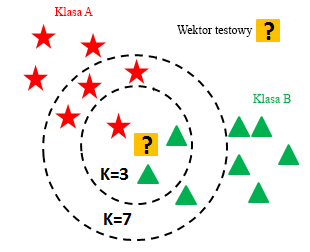
\includegraphics[width=10cm]{Obrazy/klasyfikacjaKNN.jpg}
        \caption{Przykład klasyfikacji KNN~\cite{KNNObraz}.}
        \label{fig.klasyfikacjaKNN}
    \end{figure}

    Na Rysunku \ref{fig.klasyfikacjaKNN} wyróżnione są wektory ze zbioru uczącego należące do klasy ,,A'' oraz klasy
    ,,B''. Ponadto jest na środku Rysunku \ref{fig.klasyfikacjaKNN} znajduje się wektor, który ma zostać
    sklasyfikowany do jednej z wyżej wymienionych klas.
    Dla parametru ,,k'' równego 3 wektor testowy zostanie przypisany do klasy ,,B'', gdyż z 3 najbliższych wektorów 2
    należą do klasy ,,B''. W przypadku, gdy parametr ,,k'' będzie równy 7 wektor testowy zostanie przypisany do klasy
    ,,A''. Z pośród siedmiu najbliższych sąsiadów 4 należą do klasy ,,A'', natomiast 3 do klasy ,,B''.

    Wybór parametru $k$ jest zależny od rodzaju danych. Im większa wartość $k$ tym mniejszy wpływ szumu podczas
    klasyfikacji. Szum określa błędne dane w zbiorze uczącym. Istnieją metody dobierające optymalną wartość $k$ dla
    danego zbioru uczącego. Do jednej z tych metod należy optymalizacja hiperparametryczna.

    Na końcu Sekcji \ref{subsec:zastosowanie-w-projekcie} został przedstawiony sposób, w jaki generowany jest zbiór
    uczący.
    Szacowanie wieku metodą KNN w pierwszym kroku polega na stworzeniu wektoru, który został opisany
    Wzorem \ref{wzor.hogKnn}.
    Następnym krokiem jest przydzielenie danego wektoru do klasy (wieku).

    W Sekcji \ref{ch:badania} zostaną przybliżone metody przeprowadzanie badań oraz ich wyniki.

    \chapter{Badania}\label{ch:badania}
    \section{Środowisko badań}\label{sec:środowisko-pracy}
    %napisac z czego korzystano
    %czyli matlab
    %    do czego byl uzywany matlab a do czego Intellij
    %intellij
    %jakie biblioteki uzywano z jaka dokladnocia liczono
    %    jakich technologii uzywano np. log4j do logowania
    \section{Wykrywanie zmarszczek przez detektor Canny}\label{sec:wykrywanie-krawędzi-przez-detektor-canny}
    %Ustalone parametry
    %    Tutaj mogą być zdjęcia jak to wygladalo, jakie były problemy np, ze wykrywalo wlosy, ze blednie wykrywalo itp
    \section{Statystyki z działania programu}\label{sec:statystyki-z-działania-programu}
    %opisywac nie tylko wyniki ale tez posrednio co tam lecialo, statystyki, szybkosc dzialania (sredni czas
    %    przetwarzania), zajetosc pamieci
    % napisac cos ile bylo zdjec w zbiorze danych, ile przeszlo walidacje.
    %przykladowe dane generowane przez metode glowna


    %dzialanie poszczegolnych czesci algorytmu
    %wykrywanie twarzy, oczu itd. tutaj beda zdjecia
    %logi z dzialania
    \section{Porównanie metod}
    %Skad wzielismy dane testowe
    %porownanie metod testowych
    %http://edu.pjwstk.edu.pl/wyklady/adn/scb/wyklad9/w9.htm
    %    Wstep jakie metody porownano i co tam zmieniano
    \subsection{Metoda bazowa}
    %parametry takie i takie i jakie wyniki daly zmiany o ile procent sie polepszyl lub pogorszyl MAE
    \subsection{Metoda 1}
    \subsection{Metoda 2}
    \subsection{Metoda 3}
    \section{Podsumowanie}
    \section{Wnioski}
    % za maly zbior danych testowych byc moze dlatego takie slabe wyniki?



    %troche logow z aplikacji
    %casy co sie dzialo jak nie wykryto twarzy, czy czesci twarzy wrac z logami
    %pomiar czyli ile danych przypomniec sie o mae.

    \chapter{Podsumowanie}\label{ch:podsumowanie}
    %todo poprawic bibliografie


    %%%%%%%%%%%%%%%%%%%%%%%%%%%%%%%%%%%%%%%%%%
    \backmatter
    \pagenumbering{Roman}
    \stepcounter{stronyPozaNumeracja}
    \setcounter{page}{\value{stronyPozaNumeracja}}

    \pagestyle{tylkoNumeryStron}

    %%%%%%%%%%% bibliografia %%%%%%%%%%%%
    \bibliographystyle{plplain}
    \bibliography{bibliografia}

    %%%%%%%%%  DODATKI %%%%%%%%%%%%%%%%%%%

    \begin{appendices}


        \chapter*{Dokumentacja techniczna}

        \chapter*{Spis skrótów i symboli}

        \begin{itemize}
            \item[FCM] \ang{Fuzzy C-means} - metoda klasteryzacji miękkiej (rozmytego).
            \item[HOG] \ang{Histograms of Oriented Gradients} - metoda generacji deskryptora obrazu
            \item[KNN] \ang{ k-nearest neighbors} - algorytm regresji lub klasyfikacji.
        \end{itemize}




        \chapter*{Zawartość dołączonej płyty}

        Do pracy dołączona jest płyta CD z~następującą zawartością:
        \begin{itemize}
            \item praca w~formacie \texttt{pdf},
            \item źródła programu,
            \item zbiory danych użyte w~eksperymentach.
        \end{itemize}

        \listoffigures
        \listoftables

    \end{appendices}


\end{document}


%% Finis coronat opus.